\documentclass{article}\usepackage[]{graphicx}\usepackage[]{xcolor}
% maxwidth is the original width if it is less than linewidth
% otherwise use linewidth (to make sure the graphics do not exceed the margin)
\makeatletter
\def\maxwidth{ %
  \ifdim\Gin@nat@width>\linewidth
    \linewidth
  \else
    \Gin@nat@width
  \fi
}
\makeatother

\definecolor{fgcolor}{rgb}{0.345, 0.345, 0.345}
\newcommand{\hlnum}[1]{\textcolor[rgb]{0.686,0.059,0.569}{#1}}%
\newcommand{\hlstr}[1]{\textcolor[rgb]{0.192,0.494,0.8}{#1}}%
\newcommand{\hlcom}[1]{\textcolor[rgb]{0.678,0.584,0.686}{\textit{#1}}}%
\newcommand{\hlopt}[1]{\textcolor[rgb]{0,0,0}{#1}}%
\newcommand{\hlstd}[1]{\textcolor[rgb]{0.345,0.345,0.345}{#1}}%
\newcommand{\hlkwa}[1]{\textcolor[rgb]{0.161,0.373,0.58}{\textbf{#1}}}%
\newcommand{\hlkwb}[1]{\textcolor[rgb]{0.69,0.353,0.396}{#1}}%
\newcommand{\hlkwc}[1]{\textcolor[rgb]{0.333,0.667,0.333}{#1}}%
\newcommand{\hlkwd}[1]{\textcolor[rgb]{0.737,0.353,0.396}{\textbf{#1}}}%
\let\hlipl\hlkwb

\usepackage{framed}
\makeatletter
\newenvironment{kframe}{%
 \def\at@end@of@kframe{}%
 \ifinner\ifhmode%
  \def\at@end@of@kframe{\end{minipage}}%
  \begin{minipage}{\columnwidth}%
 \fi\fi%
 \def\FrameCommand##1{\hskip\@totalleftmargin \hskip-\fboxsep
 \colorbox{shadecolor}{##1}\hskip-\fboxsep
     % There is no \\@totalrightmargin, so:
     \hskip-\linewidth \hskip-\@totalleftmargin \hskip\columnwidth}%
 \MakeFramed {\advance\hsize-\width
   \@totalleftmargin\z@ \linewidth\hsize
   \@setminipage}}%
 {\par\unskip\endMakeFramed%
 \at@end@of@kframe}
\makeatother

\definecolor{shadecolor}{rgb}{.97, .97, .97}
\definecolor{messagecolor}{rgb}{0, 0, 0}
\definecolor{warningcolor}{rgb}{1, 0, 1}
\definecolor{errorcolor}{rgb}{1, 0, 0}
\newenvironment{knitrout}{}{} % an empty environment to be redefined in TeX

\usepackage{alltt}
\usepackage[italian]{babel}
\usepackage[T1]{fontenc}

\title{NMC - Foundations of Statistical Modelling}
\author{Lorenzo Baiardi}
\date{19 Aprile 2023}
\IfFileExists{upquote.sty}{\usepackage{upquote}}{}
\begin{document}

\maketitle

\clearpage

\tableofcontents

\clearpage


\section{Introduzione}
  In questo elaborato andremo a studiare l'effetto delle attività e delle
  condizioni di salute di un individuo per la prevenzione di problemi 
  cardiovascolari. Andremo a visualizzare e considerare modelli specifici,
  differenze che sono presenti tra le diverse categorie e quanto queste categorie
  possono influire sulla presenza o meno di un problema cardiovascolare.


\section{Visualizzazione del Dataset} 
  Per lo studio di questo fenomeno utilizzeremo il Dataset fornito: 
  $\emph{Sjolander et al.(2009)}$
  Il Dataset fornisce un campione di numerosità: n = 33327 osservazioni. 
  
\begin{knitrout}
\definecolor{shadecolor}{rgb}{0.969, 0.969, 0.969}\color{fgcolor}\begin{kframe}
\begin{alltt}
\hlkwd{load}\hlstd{(}\hlstr{"../nmc.RData"}\hlstd{)}
\hlkwd{str}\hlstd{(nmc)}
\end{alltt}
\begin{verbatim}
## 'data.frame':	33327 obs. of  8 variables:
##  $ sex    : chr  "Male" "Female" "Male" "Female" ...
##  $ age    : int  94 93 92 92 91 90 89 89 89 89 ...
##  $ bmi    : num  25.6 22.9 22.9 22 24.4 ...
##  $ cvd    : int  0 0 0 1 0 0 0 1 0 1 ...
##  $ fitness: chr  "Just as good" "Much Worse" "A bit better" "Just as good" ...
##  $ pa     : int  0 1 1 0 0 0 0 0 0 0 ...
##  $ smoke  : chr  "NO" "NO" "Former" "Former" ...
##  $ alc    : chr  "Medium" "Low" "Never" "Never" ...
\end{verbatim}
\end{kframe}
\end{knitrout}
 
  \subsection{Variabili}
    Analizziamo le variabili che sono presenti nel Dataset.
    \begin{itemize}
      \item CVD: variabile d'interesse.
        \begin{enumerate}
          \setcounter{enumi}{-1}
          \item Nessun problema cardiovascolare
          \item Uno o più problemi cardiovascolari
        \end{enumerate}
      \item SEX: rappresenta il genere dell'individuo.
        \begin{itemize}
          \item Male
          \item Female
        \end{itemize}
      \item AGE: età dell'individuo.
      \item BMI: Body Mass Index, valore dicotomizzato.
        \begin{enumerate}
          \setcounter{enumi}{-1}
          \item BMI $< 30$
          \item BMI $\ge 30$ 
        \end{enumerate}
      \item FITNESS: stato di salute dell'individuo.
        \begin{enumerate}
          \item Much Worse 
          \item Little Worse
          \item Just as good
          \item A bit better
          \item Much better
        \end{enumerate}
      \item PA: Attività Fisica.
        \begin{enumerate}
          \setcounter{enumi}{-1}
          \item high-level exerciser 
          \item low-level exerciser
        \end{enumerate}
      \item SMOKE: tipologia di fumatore.
        \begin{itemize}
          \item NO 
          \item Former
          \item Current
        \end{itemize}
      \item ALCHOL: frequenza nel consumo di alchol dell'individuo.
        \begin{enumerate}
          \item Never 
          \item Low
          \item Medium
          \item High
        \end{enumerate}
    \end{itemize}
  
    Per una maggiore comprensione del problema, convertiremo alcune variabili di
    tipo categoriale in variabili di tipo ordinale per la valutazione di 
    quest ultime durante l'analisi.
    Di seguito mostreremo la legenda utilizzata.
    
\begin{knitrout}
\definecolor{shadecolor}{rgb}{0.969, 0.969, 0.969}\color{fgcolor}\begin{kframe}
\begin{alltt}
\hlcom{#LEGENDA:}
\hlcom{#Fitness: 1-MUCH WORSE, 2-LITTLE WORSE, 3-JUST AS GOOD, }
\hlcom{#         4-A BIT BETTER, 5-MUCH BETTER}
\hlcom{#Alchol: 1-NEVER, 2-LOW, 3-MEDIUM, 4-HIGH}
\hlcom{#Smoke: 1-NO, 2-FORMER, 3-CURRENT}
\hlcom{#BMI: 0-<30, 1->=30}

\hlstd{c.fit} \hlkwb{=} \hlkwd{c}\hlstd{(}\hlstr{'Much Worse'}\hlstd{,} \hlstr{'Little Worse'}\hlstd{,} \hlstr{'Just as good'}\hlstd{,}
            \hlstr{'A bit better'}\hlstd{,} \hlstr{'Much better'}\hlstd{)}
\hlstd{c.alc} \hlkwb{=}  \hlkwd{c}\hlstd{(}\hlstr{'Never'}\hlstd{,} \hlstr{'Low'}\hlstd{,} \hlstr{'Medium'}\hlstd{,} \hlstr{'High'}\hlstd{)}
\hlstd{c.smoke} \hlkwb{=} \hlkwd{c}\hlstd{(}\hlstr{'NO'}\hlstd{,} \hlstr{'Former'}\hlstd{,} \hlstr{'Current'}\hlstd{)}

\hlcom{#BMI dicotomizzata}
\hlstd{bmi} \hlkwb{=} \hlstd{nmc}\hlopt{$}\hlstd{bmi}
\hlstd{nmc}\hlopt{$}\hlstd{bmi} \hlkwb{=} \hlkwd{as.numeric}\hlstd{(nmc}\hlopt{$}\hlstd{bmi}\hlopt{>=}\hlnum{30}\hlstd{)}

\hlcom{#Variabili ordinali}
\hlstd{fitness} \hlkwb{<-} \hlstd{nmc}\hlopt{$}\hlstd{fitness}
\hlstd{nmc}\hlopt{$}\hlstd{fitness} \hlkwb{=} \hlkwd{as.numeric}\hlstd{(}\hlkwd{ordered}\hlstd{(nmc}\hlopt{$}\hlstd{fitness, c.fit))}
\hlstd{nmc}\hlopt{$}\hlstd{alc} \hlkwb{=} \hlkwd{as.numeric}\hlstd{(}\hlkwd{ordered}\hlstd{(nmc}\hlopt{$}\hlstd{alc, c.alc))}
\hlstd{smoke.ord} \hlkwb{<-} \hlkwd{as.numeric}\hlstd{(}\hlkwd{ordered}\hlstd{(nmc}\hlopt{$}\hlstd{smoke, c.smoke))}

\hlkwd{str}\hlstd{(nmc)}
\end{alltt}
\begin{verbatim}
## 'data.frame':	33327 obs. of  8 variables:
##  $ sex    : chr  "Male" "Female" "Male" "Female" ...
##  $ age    : int  94 93 92 92 91 90 89 89 89 89 ...
##  $ bmi    : num  0 0 0 0 0 0 0 0 1 0 ...
##  $ cvd    : int  0 0 0 1 0 0 0 1 0 1 ...
##  $ fitness: num  3 1 4 3 4 4 4 4 4 4 ...
##  $ pa     : int  0 1 1 0 0 0 0 0 0 0 ...
##  $ smoke  : chr  "NO" "NO" "Former" "Former" ...
##  $ alc    : num  3 2 1 1 3 2 1 3 3 1 ...
\end{verbatim}
\end{kframe}
\end{knitrout}
    
  \subsection{Tabella delle Frequenze}
    Visualizziamo la tabella delle frequenze.

    
\begin{knitrout}
\definecolor{shadecolor}{rgb}{0.969, 0.969, 0.969}\color{fgcolor}\begin{kframe}
\begin{alltt}
\hlcom{#Tabella delle Frequenze del Dataset}
\hlkwd{ftable}\hlstd{(sex}\hlopt{+}\hlstd{bmi}\hlopt{+}\hlstd{pa} \hlopt{~} \hlstd{cvd}\hlopt{+}\hlstd{smoke}\hlopt{+}\hlstd{alc}\hlopt{+}\hlstd{fitness, nmc.bn)}
\end{alltt}
\begin{verbatim}
##                       sex    0                   1               
##                       bmi    0         1         0         1     
##                       pa     0    1    0    1    0    1    0    1
## cvd smoke alc fitness                                            
## 0   1     1   1             26   11   19   10   10    3    1    0
##               2            203   36   42   10   63   21   10    1
##               3            974   77  100    8  244   30   12    1
##               4            657   19   41    0  336   18    5    1
##               5            237    1    9    0  180    4    2    0
##           2   1             79   26   37   13   29    7    9    6
##               2            600  129  133   18  183   52   23   13
##               3           3073  254  231   16  755   87   46    4
##               4           2467   47   78    3  991   34   19    1
##               5            842    6   20    0  603   12    3    1
##           3   1             24    9   14    4   19   10    7    3
##               2            202   42   38    9  120   47   20    5
##               3           1254  105   76   11  671   94   36    8
##               4           1281   29   32    2 1003   33   24    0
##               5            424    3    2    0  526    6    5    0
##           4   1              2    0    0    0    3    2    0    0
##               2              1    2    2    0    8    4    4    0
##               3             30    5    1    0   41    5    4    0
##               4             43    0    1    0   49    5    3    0
##               5             12    0    0    0   42    0    1    0
##     2     1   1              2    4    5    3    2    2    0    1
##               2             16    5   10    2    5    3    0    1
##               3             79   14   17    1   31    1    6    0
##               4             61    0    8    0   27    4    3    0
##               5             34    0    0    0   12    0    0    0
##           2   1             34   17   16   10    9    7    8    4
##               2            180   40   66   12   37   16   12    2
##               3            982   67  122    8  243   37   26    5
##               4            777   23   28    0  302   13   14    0
##               5            282    1    3    1  122    0    4    1
##           3   1             10    5    9    7    8    5    6    3
##               2            128   26   25    8   82   32   27   10
##               3            830   80   56    5  505   53   45    9
##               4            802   14   22    2  668   23   30    2
##               5            276    2    3    0  290    2    4    0
##           4   1              3    0    0    0    2    1    0    0
##               2              4    0    0    0    2    2    0    0
##               3             38    2    3    0   41    6    5    1
##               4             28    2    1    0   54    2    5    0
##               5             12    0    0    0   21    0    0    0
##     3     1   1              4    1    1    0    2    1    0    1
##               2             11    6    6    0    2    2    2    0
##               3             30    1    3    0    5    1    1    0
##               4              6    1    0    0    3    0    0    0
##               5              5    0    0    0    4    0    0    0
##           2   1             25    8   12    3    6    2    4    2
##               2            163   43   25    9   25    4    2    1
##               3            438   36   21    1   84    9    5    1
##               4            188    4    8    1   48    1    1    0
##               5             52    0    2    0   18    0    0    0
##           3   1              9    8    6    2   10    6    2    1
##               2             72   20   16    3   46   15    1    2
##               3            279   30   14    3  139   24   11    0
##               4            198    8    5    0  115    4    3    0
##               5             48    0    2    0   28    0    0    0
##           4   1              0    0    0    1    0    2    0    0
##               2              4    1    0    0    5    0    1    0
##               3             11    3    1    0   13    0    1    0
##               4              9    1    1    0    4    0    1    0
##               5              7    0    0    0    5    1    0    0
## 1   1     1   1              4    2    2    0    0    0    0    1
##               2              6    2    7    0    5    1    0    0
##               3             50    6   11    1   28    0    3    0
##               4             47    0    3    0   50    3    1    0
##               5             18    0    0    0   14    0    0    0
##           2   1              2    2    1    0    0    1    0    0
##               2             24    3    6    2    9    3    3    1
##               3             96    4   15    2   50    5    2    0
##               4             82    2    2    0   68    2    0    0
##               5             34    0    1    0   25    0    0    0
##           3   1              0    0    0    0    2    0    0    0
##               2             10    0    3    0    4    1    3    0
##               3             34    4    6    0   44    7    4    1
##               4             45    0    4    0   90    2    5    0
##               5             17    1    2    0   51    0    1    0
##           4   1              1    0    0    0    0    0    0    0
##               2              0    0    0    0    1    1    0    0
##               3              5    0    1    0    4    0    1    0
##               4              5    0    0    0    4    1    1    0
##               5              2    0    0    0    5    0    0    0
##     2     1   1              0    0    1    0    0    0    0    0
##               2              0    0    0    0    2    1    0    1
##               3              4    0    0    0   11    0    0    0
##               4              2    0    0    0    5    1    0    0
##               5              1    0    0    0    3    0    0    0
##           2   1              1    1    1    2    0    1    0    0
##               2              5    1    4    0    2    0    0    1
##               3             23    3    2    0   36    3    1    0
##               4             22    1    5    0   46    1    2    0
##               5              8    0    0    0   18    0    0    0
##           3   1              1    2    0    1    1    0    0    2
##               2              4    0    2    0   12    2    3    4
##               3             16    1    1    1   58    4    2    2
##               4             27    1    0    0   72    1    4    0
##               5              5    0    0    0   18    0    2    0
##           4   1              0    0    0    0    0    0    0    0
##               2              0    0    0    0    1    0    0    0
##               3              1    0    0    0    4    1    1    1
##               4              0    0    0    0    6    0    0    0
##               5              2    0    0    0    3    0    0    0
##     3     1   1              0    0    0    0    0    0    0    0
##               2              0    0    0    0    1    0    0    0
##               3              1    0    0    0    3    1    0    0
##               4              0    0    0    0    0    0    0    0
##               5              0    0    0    0    0    0    0    0
##           2   1              1    0    0    0    0    1    0    0
##               2              3    1    0    0    1    2    0    0
##               3             11    1    0    0   10    1    0    0
##               4              5    0    0    0    4    0    0    0
##               5              3    0    0    0    0    1    0    0
##           3   1              2    0    0    0    0    0    0    0
##               2              2    1    0    0    3    0    1    0
##               3              8    2    0    0   17    0    0    0
##               4              2    0    0    0   14    0    0    0
##               5              1    0    0    0    4    0    0    0
##           4   1              0    0    0    1    0    0    0    0
##               2              0    0    0    0    0    0    0    0
##               3              1    0    0    0    4    0    0    0
##               4              0    0    0    0    3    0    0    0
##               5              1    0    0    0    1    0    0    0
\end{verbatim}
\end{kframe}
\end{knitrout}
    
\clearpage




\section{Regressioni Logistiche Semplici}
  Dato che stiamo analizzando un problema che presenta come variabile di 
  risposta una variabile binaria (CVD), utilizzeremo la regressione logistica, 
  implementata in R tramite la funzione glm().
  Per prima cosa analizzeremo le regressioni logistiche semplici delle singole
  variabili presenti nel Dataset, visualizzandone il loro comportamento verso la
  nostra variabile di risposta.
  
  \subsection{Age}
\begin{knitrout}
\definecolor{shadecolor}{rgb}{0.969, 0.969, 0.969}\color{fgcolor}\begin{kframe}
\begin{alltt}
\hlcom{#Age}
\hlstd{fit.age} \hlkwb{<-} \hlkwd{glm}\hlstd{(cvd}\hlopt{~}\hlstd{age,} \hlkwc{family}\hlstd{=binomial,} \hlkwc{data}\hlstd{=nmc)}
\hlkwd{summary}\hlstd{(fit.age)}
\end{alltt}
\begin{verbatim}
## 
## Call:
## glm(formula = cvd ~ age, family = binomial, data = nmc)
## 
## Deviance Residuals: 
##     Min       1Q   Median       3Q      Max  
## -1.3868  -0.3530  -0.2052  -0.0986   3.5606  
## 
## Coefficients:
##              Estimate Std. Error z value Pr(>|z|)    
## (Intercept) -8.179700   0.151662  -53.93   <2e-16 ***
## age          0.092122   0.002345   39.28   <2e-16 ***
## ---
## Signif. codes:  0 '***' 0.001 '**' 0.01 '*' 0.05 '.' 0.1 ' ' 1
## 
## (Dispersion parameter for binomial family taken to be 1)
## 
##     Null deviance: 13400  on 33326  degrees of freedom
## Residual deviance: 11150  on 33325  degrees of freedom
## AIC: 11154
## 
## Number of Fisher Scoring iterations: 7
\end{verbatim}
\end{kframe}
\end{knitrout}
    
    \begin{itemize}
      \item L'età influenza positivamente l'insorgenza di un problema 
            cardiovascolare, con valore stimato: AGE $\sim$ 0.092. 
      \item La variabile AGE è molto significativa secondo il \emph{p-value}.
    \end{itemize}
    
    Stampiamo ora il Boxplot per valutare l'età delle persone che presentano
    o meno un problema cardiovascolare.
    
\begin{knitrout}
\definecolor{shadecolor}{rgb}{0.969, 0.969, 0.969}\color{fgcolor}\begin{kframe}
\begin{alltt}
\hlcom{#Boxplot}
\hlkwd{boxplot}\hlstd{(age}\hlopt{~}\hlstd{cvd,} \hlkwc{xlab}\hlstd{=}\hlstr{"CVD"}\hlstd{,} \hlkwc{ylab}\hlstd{=}\hlstr{"AGE"}\hlstd{,} \hlkwc{data}\hlstd{=nmc)}
\end{alltt}
\end{kframe}
\includegraphics[width=\maxwidth]{figure/RLS_Age_Boxplot-1} 
\end{knitrout}
    
    \begin{itemize}
      \item Il Boxplot ci mostra come la media delle persone che hanno problemi
            cardiovascolari, all'interno del Dataset, è quella della fascia
            tra i 60 e 80 anni.
      \item La media delle persone che non hanno un problema cardiovascolare è
            quella tra i 40 e 60 anni.
      \item I problemi cardiovascolari sono più frequenti nella fascia anziana
            della popolazione.
    \end{itemize}
    
    Eseguiamo il plot del modello con la sola variabile AGE.\par
    Modello: CVD $\sim$ AGE.
    
\begin{knitrout}
\definecolor{shadecolor}{rgb}{0.969, 0.969, 0.969}\color{fgcolor}\begin{kframe}
\begin{alltt}
\hlcom{#Plot}
\hlstd{pstima.age} \hlkwb{<-} \hlstd{fit.age}\hlopt{$}\hlstd{fitted.values}
\hlkwd{plot}\hlstd{(nmc}\hlopt{$}\hlstd{age, nmc}\hlopt{$}\hlstd{cvd,} \hlkwc{xlab}\hlstd{=}\hlstr{"AGE"}\hlstd{,} \hlkwc{ylab}\hlstd{=}\hlstr{"CVD"}\hlstd{)}
\hlkwd{lines}\hlstd{(}\hlkwd{sort}\hlstd{(nmc}\hlopt{$}\hlstd{age),pstima.age[}\hlkwd{order}\hlstd{(nmc}\hlopt{$}\hlstd{age)],}\hlkwc{lwd}\hlstd{=}\hlnum{3}\hlstd{,}\hlkwc{col}\hlstd{=blue)}
\end{alltt}
\end{kframe}
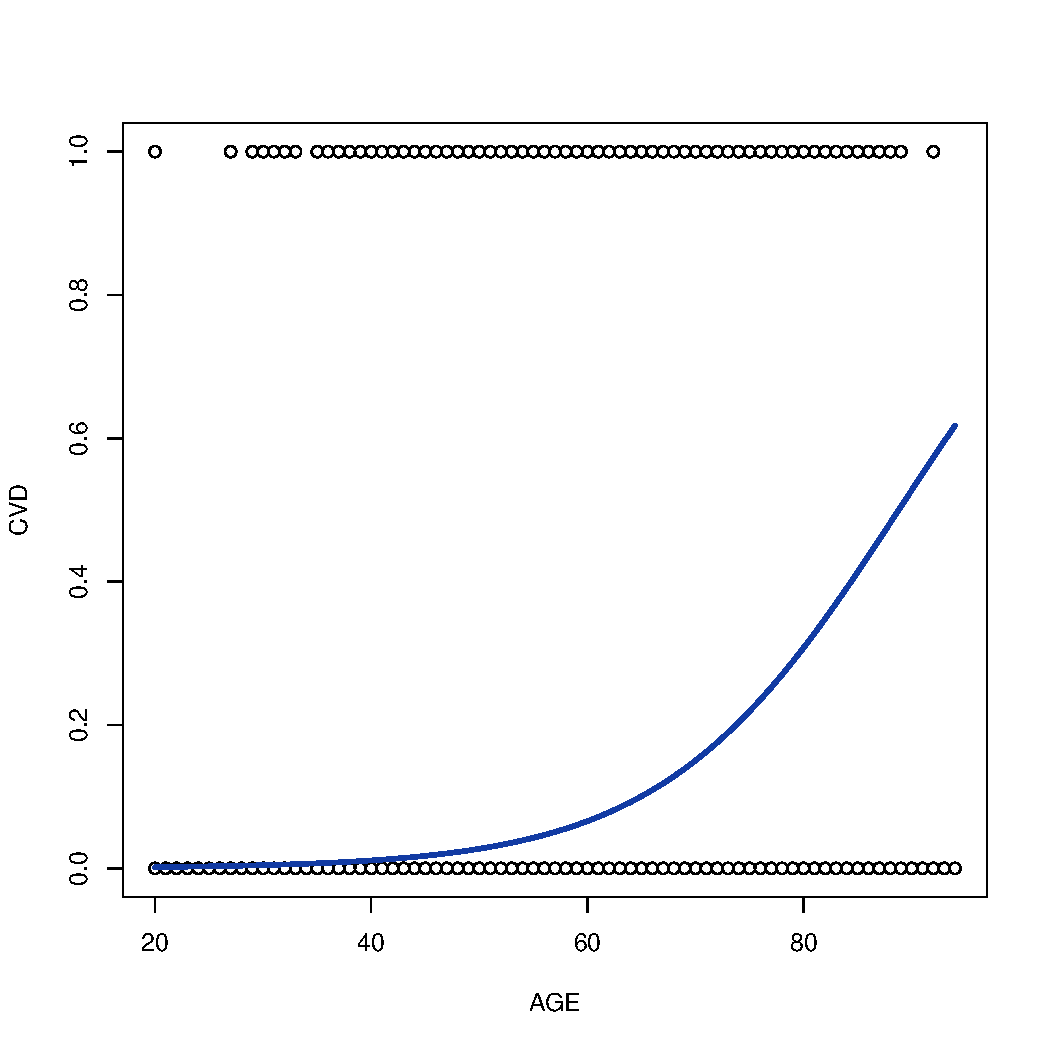
\includegraphics[width=\maxwidth]{figure/RLS_Age_Plot-1} 
\end{knitrout}
    
    Il modello e il grafico suggeriscono come, all'aumentare dell'età, ci sia un 
    aumento esponenziale nelle probabilità nell'incorrere in un problema 
    cardiovascolare. In particolare possiamo notare, come visualizzato anche dal
    Boxplot, che superata la soglia dei 40 anni si ha un notevole aumento nella
    probabilità di CVD, confermando quindi come questo problema sia legato
    principalmente ad un fattore di età.
  
  \clearpage
  
  \subsection{Sex}
\begin{knitrout}
\definecolor{shadecolor}{rgb}{0.969, 0.969, 0.969}\color{fgcolor}\begin{kframe}
\begin{alltt}
\hlcom{#Regressioni logistiche semplici}
\hlcom{#Sex}
\hlstd{fit.sex} \hlkwb{<-} \hlkwd{glm}\hlstd{(cvd}\hlopt{~}\hlstd{sex,} \hlkwc{family}\hlstd{=binomial,} \hlkwc{data}\hlstd{=nmc)}
\hlkwd{summary}\hlstd{(fit.sex)}
\end{alltt}
\begin{verbatim}
## 
## Call:
## glm(formula = cvd ~ sex, family = binomial, data = nmc)
## 
## Deviance Residuals: 
##     Min       1Q   Median       3Q      Max  
## -0.4152  -0.4152  -0.2668  -0.2668   2.5898  
## 
## Coefficients:
##             Estimate Std. Error z value Pr(>|z|)    
## (Intercept) -3.31797    0.03654  -90.80   <2e-16 ***
## sexMale      0.91004    0.05021   18.12   <2e-16 ***
## ---
## Signif. codes:  0 '***' 0.001 '**' 0.01 '*' 0.05 '.' 0.1 ' ' 1
## 
## (Dispersion parameter for binomial family taken to be 1)
## 
##     Null deviance: 13400  on 33326  degrees of freedom
## Residual deviance: 13073  on 33325  degrees of freedom
## AIC: 13077
## 
## Number of Fisher Scoring iterations: 6
\end{verbatim}
\end{kframe}
\end{knitrout}
    
    \begin{itemize}
      \item Nella regressione logistica semplice, il sesso Maschile 
            sembra aumentare notevolmente la possibilità di incorrere in un CVD 
            rispetto al sesso Femminile, con valore stimato: 
            SEX:MALE $\sim$ 0.910.
      \item La variabile SEX risulta molto significativa secondo 
            il \emph{p-value}, superando quindi il $5\%$ di significatività.
    \end{itemize}
    
    Valutiamo quanto il sesso possa influire nella presenza o meno di CVD.
    
\begin{knitrout}
\definecolor{shadecolor}{rgb}{0.969, 0.969, 0.969}\color{fgcolor}\begin{kframe}
\begin{alltt}
\hlcom{#Modello per Maschio}
\hlstd{male} \hlkwb{=} \hlstd{(nmc}\hlopt{$}\hlstd{sex}\hlopt{==}\hlstr{"Male"}\hlstd{)}
\hlstd{fit.sex.male} \hlkwb{<-} \hlkwd{glm}\hlstd{(cvd[male]}\hlopt{~}\hlstd{age[male],} \hlkwc{family}\hlstd{=binomial,} \hlkwc{data}\hlstd{=nmc)}
\hlstd{pstima.sex.male} \hlkwb{<-} \hlstd{fit.sex.male}\hlopt{$}\hlstd{fitted.values}

\hlcom{#Modello per Femmina}
\hlstd{female} \hlkwb{=} \hlstd{(nmc}\hlopt{$}\hlstd{sex}\hlopt{==}\hlstr{"Female"}\hlstd{)}
\hlstd{fit.sex.female} \hlkwb{<-} \hlkwd{glm}\hlstd{(cvd[female]}\hlopt{~}\hlstd{age[female],} \hlkwc{family}\hlstd{=binomial,} \hlkwc{data}\hlstd{=nmc)}
\hlstd{pstima.sex.female} \hlkwb{<-} \hlstd{fit.sex.female}\hlopt{$}\hlstd{fitted.values}

\hlcom{#Plot}
\hlkwd{plot}\hlstd{(nmc}\hlopt{$}\hlstd{age[male],nmc}\hlopt{$}\hlstd{cvd[male],}\hlkwc{xlab}\hlstd{=}\hlstr{"AGE"}\hlstd{,}\hlkwc{ylab}\hlstd{=}\hlstr{"CVD"}\hlstd{,}\hlkwc{col}\hlstd{=azure)}
\hlkwd{points}\hlstd{(nmc}\hlopt{$}\hlstd{age[female], nmc}\hlopt{$}\hlstd{cvd[female],}\hlkwc{col}\hlstd{=pink)}
\hlkwd{lines}\hlstd{(nmc}\hlopt{$}\hlstd{age[male],pstima.sex.male,}\hlkwc{lwd}\hlstd{=}\hlnum{3}\hlstd{,}\hlkwc{col}\hlstd{=azure)}
\hlkwd{lines}\hlstd{(nmc}\hlopt{$}\hlstd{age[female],pstima.sex.female,}\hlkwc{lwd}\hlstd{=}\hlnum{3}\hlstd{,}\hlkwc{col}\hlstd{=pink)}
\hlkwd{legend}\hlstd{(}\hlkwc{x}\hlstd{=}\hlstr{"left"}\hlstd{,}\hlkwc{legend}\hlstd{=}\hlkwd{c}\hlstd{(}\hlstr{"MALE"}\hlstd{,}\hlstr{"FEMALE"}\hlstd{),}\hlkwc{fill}\hlstd{=}\hlkwd{c}\hlstd{(azure,pink))}
\end{alltt}
\end{kframe}
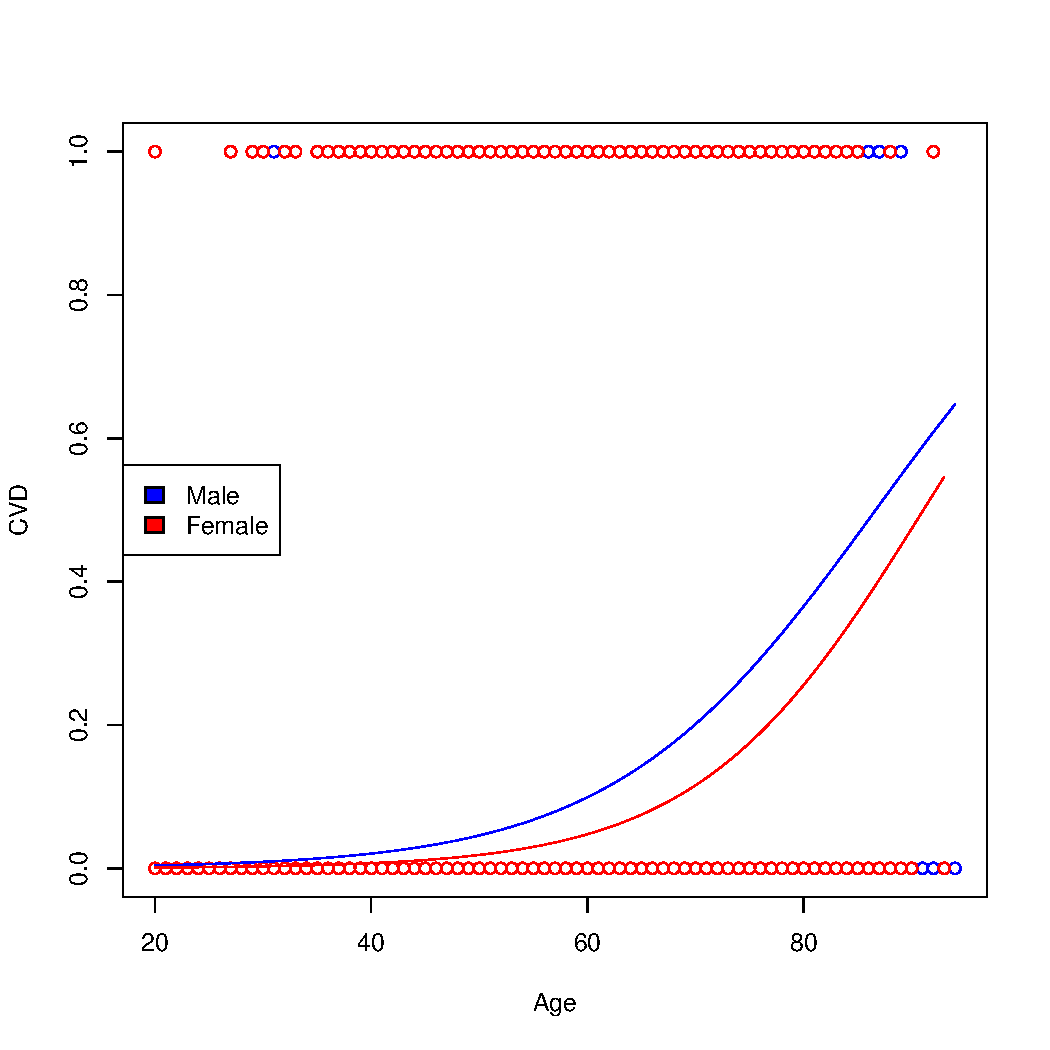
\includegraphics[width=\maxwidth]{figure/RLS_Sex_Plot-1} 
\end{knitrout}
  
    Il grafico ci conferma come il sesso maschile sia più a rischio di problemi
    cardiovascolari rispetto al sesso femminile.
  \clearpage
  \subsection{BMI}
\begin{knitrout}
\definecolor{shadecolor}{rgb}{0.969, 0.969, 0.969}\color{fgcolor}\begin{kframe}
\begin{alltt}
\hlcom{#BMI}
\hlstd{fit.bmi} \hlkwb{<-} \hlkwd{glm}\hlstd{(cvd}\hlopt{~}\hlstd{bmi,} \hlkwc{family}\hlstd{=binomial,} \hlkwc{data}\hlstd{=nmc)}
\hlkwd{summary}\hlstd{(fit.bmi)}
\end{alltt}
\begin{verbatim}
## 
## Call:
## glm(formula = cvd ~ bmi, family = binomial, data = nmc)
## 
## Deviance Residuals: 
##     Min       1Q   Median       3Q      Max  
## -0.3614  -0.3201  -0.3201  -0.3201   2.4481  
## 
## Coefficients:
##             Estimate Std. Error  z value Pr(>|z|)    
## (Intercept) -2.94542    0.02605 -113.070  < 2e-16 ***
## bmi          0.24948    0.08995    2.773  0.00555 ** 
## ---
## Signif. codes:  0 '***' 0.001 '**' 0.01 '*' 0.05 '.' 0.1 ' ' 1
## 
## (Dispersion parameter for binomial family taken to be 1)
## 
##     Null deviance: 13400  on 33326  degrees of freedom
## Residual deviance: 13393  on 33325  degrees of freedom
## AIC: 13397
## 
## Number of Fisher Scoring iterations: 5
\end{verbatim}
\end{kframe}
\end{knitrout}
    
    \begin{itemize}
      \item La variabile BMI risulta positiva nell'insorgenza di un CVD con 
            valore stimato: BMI $\sim$ 0.249.
      \item La variabile BMI risulta significativa secondo il \emph{p-value}.
    \end{itemize}
    
    Visualizziamo come il BMI possa influenzare nell'avanzamento dell'età.
    
\begin{knitrout}
\definecolor{shadecolor}{rgb}{0.969, 0.969, 0.969}\color{fgcolor}\begin{kframe}
\begin{alltt}
\hlcom{#BMI 0}
\hlstd{bmi0} \hlkwb{=} \hlstd{(nmc}\hlopt{$}\hlstd{bmi}\hlopt{==}\hlnum{0}\hlstd{)}
\hlstd{fit.bmi.0} \hlkwb{<-} \hlkwd{glm}\hlstd{(cvd[bmi0]}\hlopt{~}\hlstd{age[bmi0],} \hlkwc{family}\hlstd{=binomial,} \hlkwc{data}\hlstd{=nmc)}
\hlstd{pstima.bmi.0} \hlkwb{<-} \hlstd{fit.bmi.0}\hlopt{$}\hlstd{fitted.values}

\hlcom{#BMI 1}
\hlstd{bmi1} \hlkwb{=} \hlstd{(nmc}\hlopt{$}\hlstd{bmi}\hlopt{==}\hlnum{1}\hlstd{)}
\hlstd{fit.bmi.1} \hlkwb{<-} \hlkwd{glm}\hlstd{(cvd[bmi1]}\hlopt{~}\hlstd{age[bmi1],} \hlkwc{family}\hlstd{=binomial,} \hlkwc{data}\hlstd{=nmc)}
\hlstd{pstima.bmi.1} \hlkwb{<-} \hlstd{fit.bmi.1}\hlopt{$}\hlstd{fitted.values}

\hlcom{#Plot}
\hlkwd{plot}\hlstd{(nmc}\hlopt{$}\hlstd{age[bmi0],nmc}\hlopt{$}\hlstd{cvd[bmi0],}\hlkwc{xlab}\hlstd{=}\hlstr{"AGE"}\hlstd{,}\hlkwc{ylab}\hlstd{=}\hlstr{"CVD"}\hlstd{,}\hlkwc{col}\hlstd{=green)}
\hlkwd{points}\hlstd{(nmc}\hlopt{$}\hlstd{age[bmi1],nmc}\hlopt{$}\hlstd{cvd[bmi1],}\hlkwc{col}\hlstd{=red)}
\hlkwd{lines}\hlstd{(nmc}\hlopt{$}\hlstd{age[bmi0],pstima.bmi.0,}\hlkwc{lwd}\hlstd{=}\hlnum{3}\hlstd{,}\hlkwc{col}\hlstd{=green)}
\hlkwd{lines}\hlstd{(nmc}\hlopt{$}\hlstd{age[bmi1],pstima.bmi.1,}\hlkwc{lwd}\hlstd{=}\hlnum{3}\hlstd{,}\hlkwc{col}\hlstd{=red)}
\hlkwd{legend}\hlstd{(}\hlkwc{x}\hlstd{=}\hlstr{"left"}\hlstd{,}\hlkwc{legend}\hlstd{=}\hlkwd{c}\hlstd{(}\hlstr{"BMI Basso"}\hlstd{,}\hlstr{"BMI Alto"}\hlstd{),}\hlkwc{fill}\hlstd{=}\hlkwd{c}\hlstd{(green,red))}
\end{alltt}
\end{kframe}
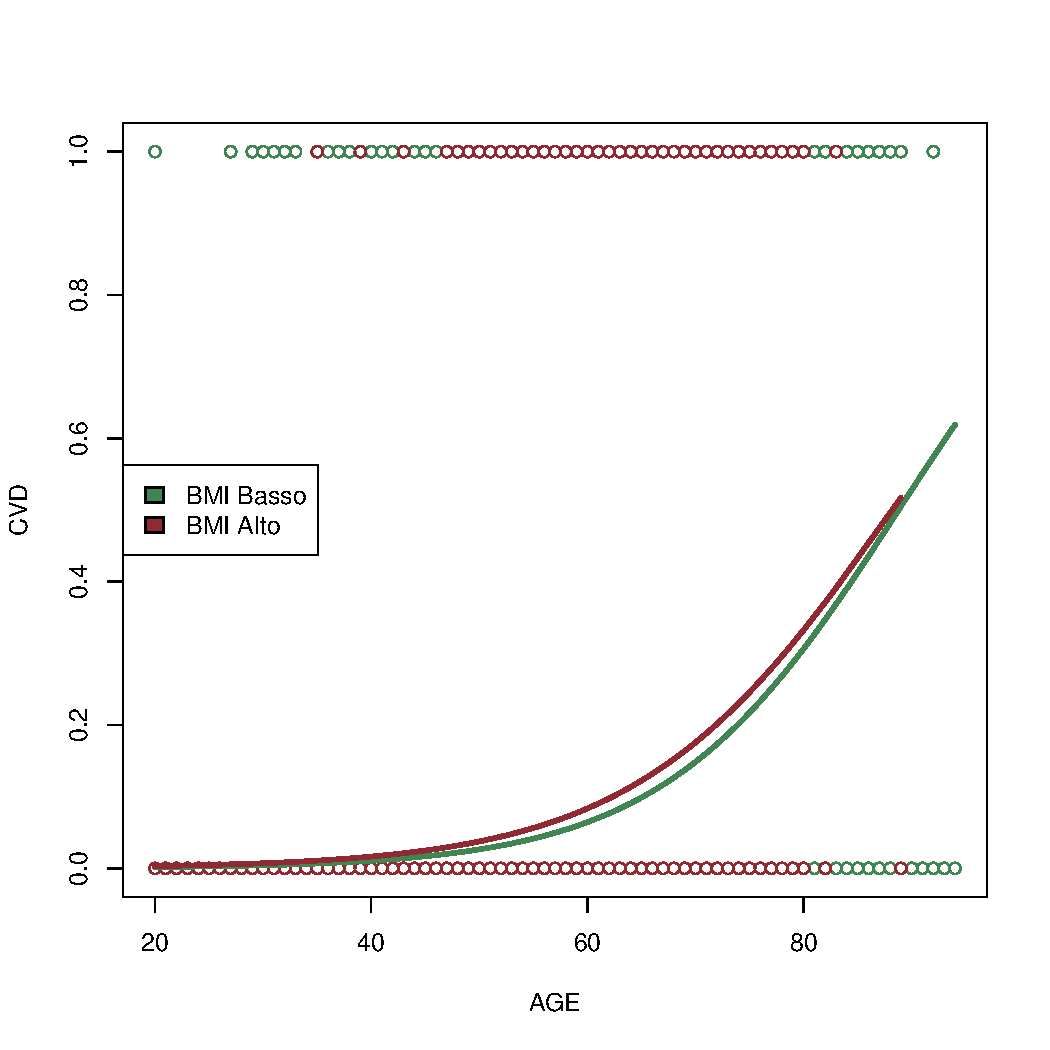
\includegraphics[width=\maxwidth]{figure/RLS_BMI_Plot-1} 
\end{knitrout}
  
    Le due curve sono molto simili tra di loro, con un leggero aumento per coloro
    che hanno un indice di massa corporea maggiore di 30.
    
  \clearpage
  
  \subsection{Fitness}
\begin{knitrout}
\definecolor{shadecolor}{rgb}{0.969, 0.969, 0.969}\color{fgcolor}\begin{kframe}
\begin{alltt}
\hlcom{#Fitness}
\hlstd{fit.fitness} \hlkwb{<-} \hlkwd{glm}\hlstd{(nmc}\hlopt{$}\hlstd{cvd} \hlopt{~} \hlstd{nmc}\hlopt{$}\hlstd{fitness,} \hlkwc{family}\hlstd{=binomial)}
\hlkwd{summary}\hlstd{(fit.fitness)}
\end{alltt}
\begin{verbatim}
## 
## Call:
## glm(formula = nmc$cvd ~ nmc$fitness, family = binomial)
## 
## Deviance Residuals: 
##     Min       1Q   Median       3Q      Max  
## -0.3438  -0.3299  -0.3166  -0.3166   2.5218  
## 
## Coefficients:
##             Estimate Std. Error z value Pr(>|z|)    
## (Intercept) -3.22195    0.09918 -32.487   <2e-16 ***
## nmc$fitness  0.08459    0.02723   3.106   0.0019 ** 
## ---
## Signif. codes:  0 '***' 0.001 '**' 0.01 '*' 0.05 '.' 0.1 ' ' 1
## 
## (Dispersion parameter for binomial family taken to be 1)
## 
##     Null deviance: 13400  on 33326  degrees of freedom
## Residual deviance: 13390  on 33325  degrees of freedom
## AIC: 13394
## 
## Number of Fisher Scoring iterations: 5
\end{verbatim}
\end{kframe}
\end{knitrout}
    
    Contrariamente a quello che ci si potesse aspettare, per il solo modello di 
    regressione logistica semplice, la variabile ordinale FITNESS risulta, anche
    se di poco, positiva e significativa per l'insorgenza di un problema 
    cardiovascolare.
    Verifichiamo quindi se ci siano delle differenze nel modello di regressione 
    logistica semplice con la variabile categoriale di FITNESS.
    
\begin{knitrout}
\definecolor{shadecolor}{rgb}{0.969, 0.969, 0.969}\color{fgcolor}\begin{kframe}
\begin{alltt}
\hlcom{#Fitness: Categoriale}
\hlstd{fit.fitness.cat} \hlkwb{<-} \hlkwd{glm}\hlstd{(nmc}\hlopt{$}\hlstd{cvd} \hlopt{~} \hlstd{fitness,} \hlkwc{family}\hlstd{=binomial)}
\hlkwd{summary}\hlstd{(fit.fitness.cat)}
\end{alltt}
\begin{verbatim}
## 
## Call:
## glm(formula = nmc$cvd ~ fitness, family = binomial)
## 
## Deviance Residuals: 
##     Min       1Q   Median       3Q      Max  
## -0.3404  -0.3404  -0.3083  -0.3083   2.4894  
## 
## Coefficients:
##                     Estimate Std. Error z value Pr(>|z|)    
## (Intercept)         -2.81935    0.04066 -69.344  < 2e-16 ***
## fitnessJust as good -0.20312    0.05783  -3.512 0.000444 ***
## fitnessLittle Worse -0.23313    0.09169  -2.542 0.011009 *  
## fitnessMuch better  -0.03049    0.07762  -0.393 0.694406    
## fitnessMuch Worse   -0.09915    0.17360  -0.571 0.567914    
## ---
## Signif. codes:  0 '***' 0.001 '**' 0.01 '*' 0.05 '.' 0.1 ' ' 1
## 
## (Dispersion parameter for binomial family taken to be 1)
## 
##     Null deviance: 13400  on 33326  degrees of freedom
## Residual deviance: 13384  on 33322  degrees of freedom
## AIC: 13394
## 
## Number of Fisher Scoring iterations: 5
\end{verbatim}
\end{kframe}
\end{knitrout}
    
    \begin{itemize}
      \item Con la variabile categoriale di FITNESS notiamo come ci sia una 
            diminuzione nell'insorgenza di CVD per tutte le categorie.
      \item Solamente le categorie FITNESS:JUSTASGOOD e FITNESS:LITTLEWORSE
            risultano significative.
    \end{itemize}
    
    Visualizziamo il comportamento della variabile FITNESS all'aumentare dell'età.
    
\begin{knitrout}
\definecolor{shadecolor}{rgb}{0.969, 0.969, 0.969}\color{fgcolor}\begin{kframe}
\begin{alltt}
\hlcom{#Fitness:MuchWorse}
\hlstd{f.mw} \hlkwb{=} \hlstd{(fitness}\hlopt{==}\hlstr{"Much Worse"}\hlstd{)}
\hlstd{fit.fitness.mw} \hlkwb{<-} \hlkwd{glm}\hlstd{(cvd[f.mw]}\hlopt{~}\hlstd{age[f.mw],}\hlkwc{family}\hlstd{=binomial,}\hlkwc{data}\hlstd{=nmc)}
\hlstd{pstima.fitness.mw} \hlkwb{<-} \hlstd{fit.fitness.mw}\hlopt{$}\hlstd{fitted.values}

\hlcom{#Fitness:LittleWorse}
\hlstd{f.lw} \hlkwb{=} \hlstd{(fitness}\hlopt{==}\hlstr{"Little Worse"}\hlstd{)}
\hlstd{fit.fitness.lw} \hlkwb{<-} \hlkwd{glm}\hlstd{(cvd[f.lw]}\hlopt{~}\hlstd{age[f.lw],}\hlkwc{family}\hlstd{=binomial,}\hlkwc{data}\hlstd{=nmc)}
\hlstd{pstima.fitness.lw} \hlkwb{<-} \hlstd{fit.fitness.lw}\hlopt{$}\hlstd{fitted.values}

\hlcom{#Fitness:Justasgood}
\hlstd{f.jg} \hlkwb{=} \hlstd{(fitness}\hlopt{==}\hlstr{"Just as good"}\hlstd{)}
\hlstd{fit.fitness.jg}\hlkwb{<-} \hlkwd{glm}\hlstd{(cvd[f.jg]}\hlopt{~}\hlstd{age[f.jg],}\hlkwc{family}\hlstd{=binomial,}\hlkwc{data}\hlstd{=nmc)}
\hlstd{pstima.fitness.jg} \hlkwb{<-} \hlstd{fit.fitness.jg}\hlopt{$}\hlstd{fitted.values}

\hlcom{#Fitness:Abitbetter}
\hlstd{f.bb} \hlkwb{=} \hlstd{(fitness}\hlopt{==}\hlstr{"A bit better"}\hlstd{)}
\hlstd{fit.fitness.bb} \hlkwb{<-} \hlkwd{glm}\hlstd{(cvd[f.bb]}\hlopt{~}\hlstd{age[f.bb],}\hlkwc{family}\hlstd{=binomial,}\hlkwc{data}\hlstd{=nmc)}
\hlstd{pstima.fitness.bb} \hlkwb{<-} \hlstd{fit.fitness.bb}\hlopt{$}\hlstd{fitted.values}

\hlcom{#Fitness:Muchbetter}
\hlstd{f.mb} \hlkwb{=} \hlstd{(fitness}\hlopt{==}\hlstr{"Much better"}\hlstd{)}
\hlstd{fit.fitness.mb} \hlkwb{<-} \hlkwd{glm}\hlstd{(cvd[f.mb]}\hlopt{~}\hlstd{age[f.mb],}\hlkwc{family}\hlstd{=binomial,}\hlkwc{data}\hlstd{=nmc)}
\hlstd{pstima.fitness.mb} \hlkwb{<-} \hlstd{fit.fitness.mb}\hlopt{$}\hlstd{fitted.values}

\hlcom{#Plot}
\hlkwd{plot}\hlstd{(nmc}\hlopt{$}\hlstd{age[f.mw],nmc}\hlopt{$}\hlstd{cvd[f.mw],}\hlkwc{xlab}\hlstd{=}\hlstr{"AGE"}\hlstd{,}\hlkwc{ylab}\hlstd{=}\hlstr{"CVD"}\hlstd{,}\hlkwc{col}\hlstd{=black)}
\hlkwd{points}\hlstd{(nmc}\hlopt{$}\hlstd{age[f.lw],nmc}\hlopt{$}\hlstd{cvd[f.lw],}\hlkwc{col}\hlstd{=red)}
\hlkwd{points}\hlstd{(nmc}\hlopt{$}\hlstd{age[f.jg],nmc}\hlopt{$}\hlstd{cvd[f.jg],}\hlkwc{col}\hlstd{=yellow)}
\hlkwd{points}\hlstd{(nmc}\hlopt{$}\hlstd{age[f.bb],nmc}\hlopt{$}\hlstd{cvd[f.bb],}\hlkwc{col}\hlstd{=orange)}
\hlkwd{points}\hlstd{(nmc}\hlopt{$}\hlstd{age[f.mb],nmc}\hlopt{$}\hlstd{cvd[f.mb],}\hlkwc{col}\hlstd{=green)}
\hlkwd{lines}\hlstd{(nmc}\hlopt{$}\hlstd{age[f.mw],pstima.fitness.mw,}\hlkwc{lwd}\hlstd{=}\hlnum{3}\hlstd{,}\hlkwc{col}\hlstd{=black)}
\hlkwd{lines}\hlstd{(nmc}\hlopt{$}\hlstd{age[f.lw],pstima.fitness.lw,}\hlkwc{lwd}\hlstd{=}\hlnum{3}\hlstd{,}\hlkwc{col}\hlstd{=red)}
\hlkwd{lines}\hlstd{(nmc}\hlopt{$}\hlstd{age[f.jg],pstima.fitness.jg,}\hlkwc{lwd}\hlstd{=}\hlnum{3}\hlstd{,}\hlkwc{col}\hlstd{=orange)}
\hlkwd{lines}\hlstd{(nmc}\hlopt{$}\hlstd{age[f.bb],pstima.fitness.bb,}\hlkwc{lwd}\hlstd{=}\hlnum{3}\hlstd{,}\hlkwc{col}\hlstd{=yellow)}
\hlkwd{lines}\hlstd{(nmc}\hlopt{$}\hlstd{age[f.mb],pstima.fitness.mb,}\hlkwc{lwd}\hlstd{=}\hlnum{3}\hlstd{,}\hlkwc{col}\hlstd{=green)}
\hlkwd{legend}\hlstd{(}\hlkwc{x}\hlstd{=}\hlstr{"left"}\hlstd{,}\hlkwc{legend}\hlstd{=}\hlkwd{c}\hlstd{(}\hlstr{"Much Worse"}\hlstd{,}\hlstr{"Little Worse"}\hlstd{,}\hlstr{"Just as good"}\hlstd{,}
       \hlstr{"A bit better"}\hlstd{,} \hlstr{"Much better"}\hlstd{),}
       \hlkwc{fill}\hlstd{=}\hlkwd{c}\hlstd{(black,red,orange,yellow,green))}
\end{alltt}
\end{kframe}
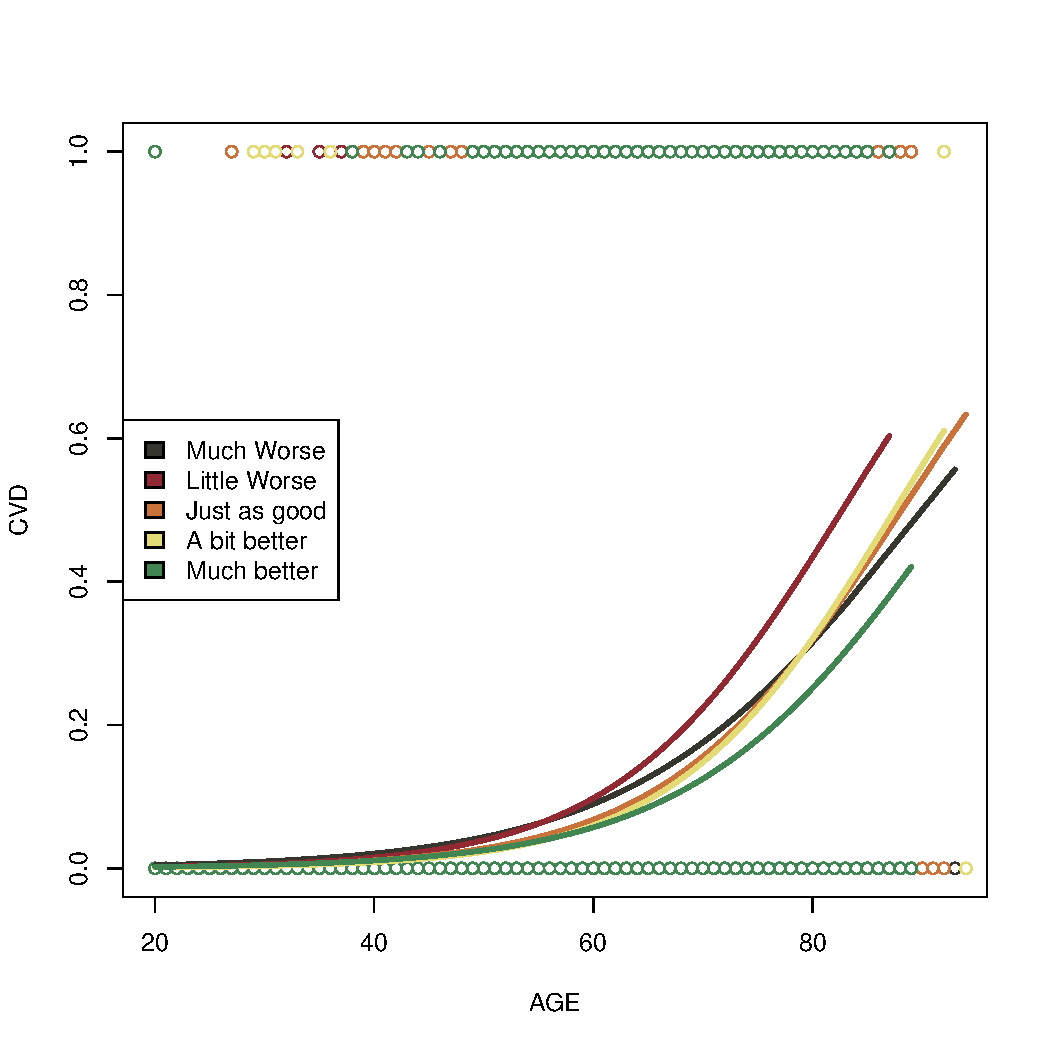
\includegraphics[width=\maxwidth]{figure/RLS_Fitness_Plot-1} 
\end{knitrout}
    
    Attraverso il grafico notiamo che la categoria FITNESS:MUCHBETTER è quella meno
    soggetta rispetto a tutte le altre. Viceversa la categoria FITNESS:LITTLEWORSE 
    ha più probabilità di incorrere in un problema cardiovascolare.
    Chi è della categoria FITNESS:MUCHWORSE ha meno probabilità rispetto alla 
    categoria FITNESS:LITTLEWORSE evidenziando come un problema cardiovascolare
    non è associato per forza a una pessima condizione di salute.
    Dobbiamo comunque considerare che la variabile FITNESS sia una variabile
    soggettiva a discrezione dell'individuo e per questo può l'idea di
    benessere può variare da persona a persona.
    In conclusione, per il solo modello di regressione logistica semplice,
    consideriamo la variabile FITNESS come significativa.
    
  \clearpage

  \subsection{PA}
\begin{knitrout}
\definecolor{shadecolor}{rgb}{0.969, 0.969, 0.969}\color{fgcolor}\begin{kframe}
\begin{alltt}
\hlcom{#PA}
\hlstd{fit.pa} \hlkwb{<-} \hlkwd{glm}\hlstd{(cvd}\hlopt{~}\hlstd{pa,} \hlkwc{family}\hlstd{=binomial,} \hlkwc{data}\hlstd{=nmc)}
\hlkwd{summary}\hlstd{(fit.pa)}
\end{alltt}
\begin{verbatim}
## 
## Call:
## glm(formula = cvd ~ pa, family = binomial, data = nmc)
## 
## Deviance Residuals: 
##     Min       1Q   Median       3Q      Max  
## -0.3242  -0.3242  -0.3242  -0.3242   2.4754  
## 
## Coefficients:
##             Estimate Std. Error  z value Pr(>|z|)    
## (Intercept) -2.91978    0.02581 -113.126   <2e-16 ***
## pa          -0.09610    0.09974   -0.963    0.335    
## ---
## Signif. codes:  0 '***' 0.001 '**' 0.01 '*' 0.05 '.' 0.1 ' ' 1
## 
## (Dispersion parameter for binomial family taken to be 1)
## 
##     Null deviance: 13400  on 33326  degrees of freedom
## Residual deviance: 13399  on 33325  degrees of freedom
## AIC: 13403
## 
## Number of Fisher Scoring iterations: 5
\end{verbatim}
\end{kframe}
\end{knitrout}
    
    Secondo la valutazione del \emph{p-value} la variabile PA, nonostante 
    influisca negativamente per la CVD, non supera il $5\%$ di significatività, 
    risultando non significativa.
    
  \subsection{Smoke}  
\begin{knitrout}
\definecolor{shadecolor}{rgb}{0.969, 0.969, 0.969}\color{fgcolor}\begin{kframe}
\begin{alltt}
\hlcom{#Smoke}
\hlstd{fit.smoke} \hlkwb{<-} \hlkwd{glm}\hlstd{(cvd}\hlopt{~}\hlstd{smoke,} \hlkwc{family}\hlstd{=binomial,} \hlkwc{data}\hlstd{=nmc)}
\hlkwd{summary}\hlstd{(fit.smoke)}
\end{alltt}
\begin{verbatim}
## 
## Call:
## glm(formula = cvd ~ smoke, family = binomial, data = nmc)
## 
## Deviance Residuals: 
##     Min       1Q   Median       3Q      Max  
## -0.3402  -0.3186  -0.3186  -0.3186   2.4946  
## 
## Coefficients:
##             Estimate Std. Error z value Pr(>|z|)    
## (Intercept) -3.06590    0.09377 -32.696   <2e-16 ***
## smokeFormer  0.24571    0.10465   2.348   0.0189 *  
## smokeNO      0.11061    0.09880   1.119   0.2629    
## ---
## Signif. codes:  0 '***' 0.001 '**' 0.01 '*' 0.05 '.' 0.1 ' ' 1
## 
## (Dispersion parameter for binomial family taken to be 1)
## 
##     Null deviance: 13400  on 33326  degrees of freedom
## Residual deviance: 13392  on 33324  degrees of freedom
## AIC: 13398
## 
## Number of Fisher Scoring iterations: 5
\end{verbatim}
\end{kframe}
\end{knitrout}
  
    \begin{itemize}
      \item Le categorie SMOKE:FORMER e SMOKE:NO sembrano influire positivamente
            sull'insorgenza di CVD.
      \item Risulta significativa solo la categoria SMOKE:FORMER con valore stimato:
            SMOKE:FORMER $\sim$ 0.246.
    \end{itemize}
    
    Verifichiamo ora il modello di regressione logistica semplice nel caso della 
    variabile ordinale SMOKE.
    
\begin{knitrout}
\definecolor{shadecolor}{rgb}{0.969, 0.969, 0.969}\color{fgcolor}\begin{kframe}
\begin{alltt}
\hlcom{#Smoke Ordinale}
\hlstd{fit.smoke.ord} \hlkwb{<-} \hlkwd{glm}\hlstd{(nmc}\hlopt{$}\hlstd{cvd} \hlopt{~} \hlstd{smoke.ord,} \hlkwc{family}\hlstd{=binomial)}
\hlkwd{summary}\hlstd{(fit.smoke.ord)}
\end{alltt}
\begin{verbatim}
## 
## Call:
## glm(formula = nmc$cvd ~ smoke.ord, family = binomial)
## 
## Deviance Residuals: 
##     Min       1Q   Median       3Q      Max  
## -0.3281  -0.3249  -0.3218  -0.3218   2.4441  
## 
## Coefficients:
##             Estimate Std. Error z value Pr(>|z|)    
## (Intercept) -2.95522    0.06099 -48.454   <2e-16 ***
## smoke.ord    0.02015    0.03893   0.518    0.605    
## ---
## Signif. codes:  0 '***' 0.001 '**' 0.01 '*' 0.05 '.' 0.1 ' ' 1
## 
## (Dispersion parameter for binomial family taken to be 1)
## 
##     Null deviance: 13400  on 33326  degrees of freedom
## Residual deviance: 13400  on 33325  degrees of freedom
## AIC: 13404
## 
## Number of Fisher Scoring iterations: 5
\end{verbatim}
\end{kframe}
\end{knitrout}
    
    \begin{itemize}
      \item La variabile ordinale SMOKE risulta positiva nell'insorgenza di CVD.
      \item Nonostante ciò la variabile SMOKE ordinale risulta non significativa
            secondo il \emph{p-value}.
    \end{itemize}
    
    Analizziamo se ci siano delle differenze tra le varie categorie di fumatori
    con l'avanzare dell'età.
    
\begin{knitrout}
\definecolor{shadecolor}{rgb}{0.969, 0.969, 0.969}\color{fgcolor}\begin{kframe}
\begin{alltt}
\hlcom{#Smoke:NO}
\hlstd{s.no} \hlkwb{=} \hlstd{(nmc}\hlopt{$}\hlstd{smoke}\hlopt{==}\hlstr{"NO"}\hlstd{)}
\hlstd{fit.smoke.no} \hlkwb{<-} \hlkwd{glm}\hlstd{(cvd[s.no]}\hlopt{~}\hlstd{age[s.no],} \hlkwc{family}\hlstd{=binomial,} \hlkwc{data}\hlstd{=nmc)}
\hlstd{pstima.smoke.no} \hlkwb{<-} \hlstd{fit.smoke.no}\hlopt{$}\hlstd{fitted.values}

\hlcom{#Smoke:Former}
\hlstd{s.f} \hlkwb{=} \hlstd{(nmc}\hlopt{$}\hlstd{smoke}\hlopt{==}\hlstr{"Former"}\hlstd{)}
\hlstd{fit.smoke.f} \hlkwb{<-} \hlkwd{glm}\hlstd{(cvd[s.f]}\hlopt{~}\hlstd{age[s.f],} \hlkwc{family}\hlstd{=binomial,} \hlkwc{data}\hlstd{=nmc)}
\hlstd{pstima.smoke.f} \hlkwb{<-} \hlstd{fit.smoke.f}\hlopt{$}\hlstd{fitted.values}

\hlcom{#Smoke:Current}
\hlstd{s.c} \hlkwb{=} \hlstd{(nmc}\hlopt{$}\hlstd{smoke}\hlopt{==}\hlstr{"Current"}\hlstd{)}
\hlstd{fit.smoke.c} \hlkwb{<-} \hlkwd{glm}\hlstd{(cvd[s.c]}\hlopt{~}\hlstd{age[s.c],} \hlkwc{family}\hlstd{=binomial,} \hlkwc{data}\hlstd{=nmc)}
\hlstd{pstima.smoke.c} \hlkwb{<-} \hlstd{fit.smoke.c}\hlopt{$}\hlstd{fitted.values}

\hlcom{#Plot}
\hlkwd{plot}\hlstd{(nmc}\hlopt{$}\hlstd{age[s.no],nmc}\hlopt{$}\hlstd{cvd[s.no],}\hlkwc{xlab}\hlstd{=}\hlstr{"AGE"}\hlstd{,}\hlkwc{ylab}\hlstd{=}\hlstr{"CVD"}\hlstd{,}\hlkwc{col}\hlstd{=green)}
\hlkwd{points}\hlstd{(nmc}\hlopt{$}\hlstd{age[s.f],nmc}\hlopt{$}\hlstd{cvd[s.f],}\hlkwc{col}\hlstd{=orange)}
\hlkwd{points}\hlstd{(nmc}\hlopt{$}\hlstd{age[s.c],nmc}\hlopt{$}\hlstd{cvd[s.c],}\hlkwc{col}\hlstd{=red)}
\hlkwd{lines}\hlstd{(nmc}\hlopt{$}\hlstd{age[s.no],pstima.smoke.no,}\hlkwc{lwd}\hlstd{=}\hlnum{3}\hlstd{,}\hlkwc{col}\hlstd{=green)}
\hlkwd{lines}\hlstd{(nmc}\hlopt{$}\hlstd{age[s.f],pstima.smoke.f,}\hlkwc{lwd}\hlstd{=}\hlnum{3}\hlstd{,}\hlkwc{col}\hlstd{=orange)}
\hlkwd{lines}\hlstd{(nmc}\hlopt{$}\hlstd{age[s.c],pstima.smoke.c,}\hlkwc{lwd}\hlstd{=}\hlnum{3}\hlstd{,}\hlkwc{col}\hlstd{=red)}
\hlkwd{legend}\hlstd{(}\hlkwc{x}\hlstd{=}\hlstr{"left"}\hlstd{,} \hlkwc{legend}\hlstd{=}\hlkwd{c}\hlstd{(}\hlstr{"NO"}\hlstd{,} \hlstr{"Former"}\hlstd{,} \hlstr{"Current"}\hlstd{),}
       \hlkwc{fill}\hlstd{=}\hlkwd{c}\hlstd{(green,orange,red))}
\end{alltt}
\end{kframe}
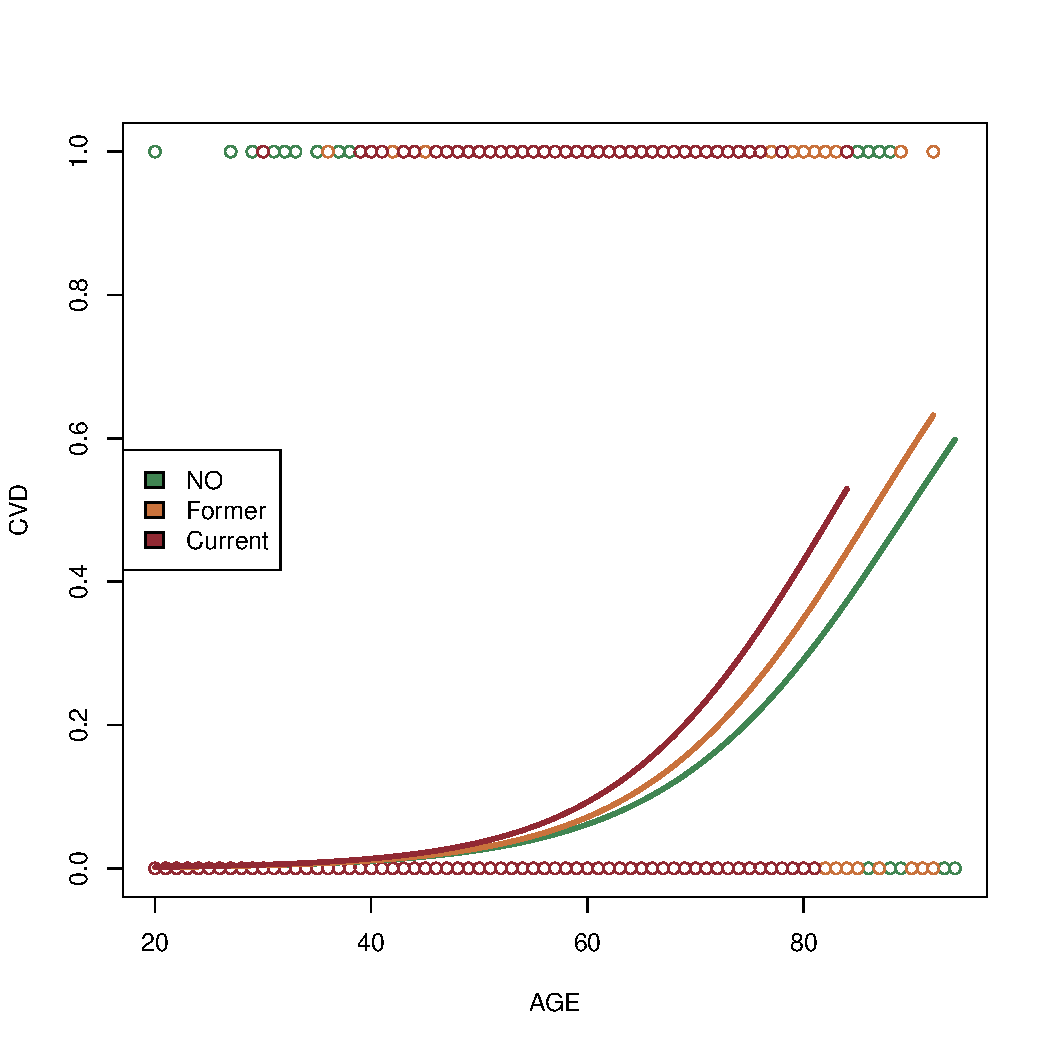
\includegraphics[width=\maxwidth]{figure/RLS_Smoke_Plot-1} 
\end{knitrout}
    
    Possiamo notare come un fumatore, rispetto alle altre categorie, abbia una
    maggiore probabilità di incorrere nella malattia con il passare del tempo.\par
    Viceversa, il non fumatore ha meno probabilità rispetto alle altre categorie di
    incorrere nella malattia.
    
  \clearpage  
    
  \subsection{Alchol}
\begin{knitrout}
\definecolor{shadecolor}{rgb}{0.969, 0.969, 0.969}\color{fgcolor}\begin{kframe}
\begin{alltt}
\hlcom{#Alchol}
\hlstd{fit.alc} \hlkwb{<-} \hlkwd{glm}\hlstd{(cvd}\hlopt{~}\hlstd{alc,} \hlkwc{family}\hlstd{=binomial,} \hlkwc{data}\hlstd{=nmc)}
\hlkwd{summary}\hlstd{(fit.alc)}
\end{alltt}
\begin{verbatim}
## 
## Call:
## glm(formula = cvd ~ alc, family = binomial, data = nmc)
## 
## Deviance Residuals: 
##     Min       1Q   Median       3Q      Max  
## -0.3241  -0.3235  -0.3230  -0.3230   2.4425  
## 
## Coefficients:
##              Estimate Std. Error z value Pr(>|z|)    
## (Intercept) -2.934597   0.084928  -34.55   <2e-16 ***
## alc          0.003563   0.035652    0.10     0.92    
## ---
## Signif. codes:  0 '***' 0.001 '**' 0.01 '*' 0.05 '.' 0.1 ' ' 1
## 
## (Dispersion parameter for binomial family taken to be 1)
## 
##     Null deviance: 13400  on 33326  degrees of freedom
## Residual deviance: 13400  on 33325  degrees of freedom
## AIC: 13404
## 
## Number of Fisher Scoring iterations: 5
\end{verbatim}
\end{kframe}
\end{knitrout}
    
    La variabile ALCHOL, secondo la valutazione del \emph{p-value}, non supera
    il $5\%$ di significatività, risultando non significativa.
  
  \subsection{Commento}
    Nei soli modelli con regressione logistica semplice abbiamo che:
    \begin{itemize}
      \item Le variabili che risultano essere significative secondo la valutazione
            del \emph{p-value} sono: SEX, AGE, BMI e FITNESS.
      \item Sempre secondo la valutazione del \emph{p-value}, le variabili che 
            invece risultano non significative sono: PA, SMOKE e ALCHOL.
      \item Le variabili SEX:MALE, AGE e BMI aumentano il rischio di CVD.
      \item La variabile FITNESS evidenzia il fatto che chi sta bene è meno
            soggetto alla problematica.
      \item Un fumatore è più soggetto alla malattia rispetto alle altre categorie.
    \end{itemize}
  
\clearpage


\section{Regressioni Logistiche Multiple}
  Consideriamo ora la regressione logistica multipla includendo tutte le variabili
  che sono presenti all'interno del Dataset, verificando quali di esse sono più 
  o meno significative.
  
  \subsection{Modello Completo}
\begin{knitrout}
\definecolor{shadecolor}{rgb}{0.969, 0.969, 0.969}\color{fgcolor}\begin{kframe}
\begin{alltt}
\hlcom{#Regressioni logistiche multiple}
\hlcom{#Modello Completo}
\hlcom{#Variabili: Sex, Age, BMI, Fitness, PA, Smoke, Alchol}
\hlstd{fit.all} \hlkwb{<-} \hlkwd{glm}\hlstd{(cvd}\hlopt{~}\hlstd{sex}\hlopt{+}\hlstd{age}\hlopt{+}\hlstd{bmi}\hlopt{+}\hlstd{fitness}\hlopt{+}\hlstd{pa}\hlopt{+}\hlstd{smoke}\hlopt{+}\hlstd{alc,} \hlkwc{data}\hlstd{=nmc,}
               \hlkwc{family}\hlstd{=binomial)}
\hlkwd{summary}\hlstd{(fit.all)}
\end{alltt}
\begin{verbatim}
## 
## Call:
## glm(formula = cvd ~ sex + age + bmi + fitness + pa + smoke + 
##     alc, family = binomial, data = nmc)
## 
## Deviance Residuals: 
##     Min       1Q   Median       3Q      Max  
## -1.5967  -0.3394  -0.1937  -0.0950   3.6484  
## 
## Coefficients:
##              Estimate Std. Error z value Pr(>|z|)    
## (Intercept) -7.475667   0.213543 -35.008  < 2e-16 ***
## sexMale      0.799132   0.054689  14.612  < 2e-16 ***
## age          0.092680   0.002446  37.896  < 2e-16 ***
## bmi          0.235120   0.096986   2.424 0.015339 *  
## fitness     -0.181741   0.031070  -5.849 4.93e-09 ***
## pa           0.035563   0.108422   0.328 0.742909    
## smokeFormer -0.332158   0.111102  -2.990 0.002793 ** 
## smokeNO     -0.374001   0.106486  -3.512 0.000444 ***
## alc         -0.056404   0.035625  -1.583 0.113368    
## ---
## Signif. codes:  0 '***' 0.001 '**' 0.01 '*' 0.05 '.' 0.1 ' ' 1
## 
## (Dispersion parameter for binomial family taken to be 1)
## 
##     Null deviance: 13400  on 33326  degrees of freedom
## Residual deviance: 10883  on 33318  degrees of freedom
## AIC: 10901
## 
## Number of Fisher Scoring iterations: 7
\end{verbatim}
\end{kframe}
\end{knitrout}
    
    Per il modello che include tutte le variabili:\\
    Modello: CVD $\sim$ SEX + AGE + BMI + FITNESS + PA + SMOKE + ALCHOL 
    \begin{itemize}
      \item Risultano essere significative, secondo il \emph{p-value}, le 
            variabili: SEX, AGE, BMI, FITNESS e SMOKE.
      \item Risultano essere non significative, non superando il $5\%$
            di significatività del \emph{p-value}, le variabili: PA e ALCHOL.
      \item I parametri stimati nella regressione logistica multipla differiscono
            da quelli presenti nelle regressioni logistiche semplici precedentemente
            analizzate.
      \item Gli errori standard non differiscono molto da quelli presenti nei
            modelli con regressione logistica semplice.
      \item La variabile SEX mostra ancora come il sesso maschile influisca 
            positivamente nella presenza di CVD con valore stimato: 
            SEX:MALE $\sim$ 0.799.
      \item Anche le variabili BMI e SMOKE mostrano un aumento nelle possibilità 
            di insorgenza di un CVD.
      \item La variabile FITNESS aumenta di significatività, rispetto
            al modello di regressione logistica semplice, riducendo la 
            probabilità di CVD con valore stimato: FITNESS $\sim$ -0.182.
    \end{itemize}
  
  \subsection{Modello Significativo}
    Dato che nel modello completo sono presenti variabili non significative,
    le andremo ad eliminare gradualmente dalla formula del modello fino ad 
    ottenere un modello con solo variabili significative.
    Iniziamo eliminando la variabile non significativa PA.
    
\begin{knitrout}
\definecolor{shadecolor}{rgb}{0.969, 0.969, 0.969}\color{fgcolor}\begin{kframe}
\begin{alltt}
\hlcom{#Modello senza PA}
\hlcom{#Variabili: Sex, Age, BMI, Fitness, Smoke, Alchol}
\hlstd{fit.npa} \hlkwb{<-} \hlkwd{glm}\hlstd{(cvd}\hlopt{~}\hlstd{sex}\hlopt{+}\hlstd{age}\hlopt{+}\hlstd{bmi}\hlopt{+}\hlstd{fitness}\hlopt{+}\hlstd{smoke}\hlopt{+}\hlstd{alc,} \hlkwc{data}\hlstd{=nmc,}
               \hlkwc{family}\hlstd{=binomial)}
\hlkwd{summary}\hlstd{(fit.npa)}
\end{alltt}
\begin{verbatim}
## 
## Call:
## glm(formula = cvd ~ sex + age + bmi + fitness + smoke + alc, 
##     family = binomial, data = nmc)
## 
## Deviance Residuals: 
##     Min       1Q   Median       3Q      Max  
## -1.5978  -0.3371  -0.1941  -0.0950   3.6471  
## 
## Coefficients:
##              Estimate Std. Error z value Pr(>|z|)    
## (Intercept) -7.462934   0.209921 -35.551  < 2e-16 ***
## sexMale      0.799887   0.054643  14.638  < 2e-16 ***
## age          0.092640   0.002442  37.930  < 2e-16 ***
## bmi          0.235857   0.096958   2.433 0.014992 *  
## fitness     -0.183877   0.030378  -6.053 1.42e-09 ***
## smokeFormer -0.332592   0.111097  -2.994 0.002756 ** 
## smokeNO     -0.374525   0.106476  -3.517 0.000436 ***
## alc         -0.056553   0.035625  -1.587 0.112413    
## ---
## Signif. codes:  0 '***' 0.001 '**' 0.01 '*' 0.05 '.' 0.1 ' ' 1
## 
## (Dispersion parameter for binomial family taken to be 1)
## 
##     Null deviance: 13400  on 33326  degrees of freedom
## Residual deviance: 10883  on 33319  degrees of freedom
## AIC: 10899
## 
## Number of Fisher Scoring iterations: 7
\end{verbatim}
\end{kframe}
\end{knitrout}
    
    Tutte le variabili che erano significative nel modello completo risultano 
    ancora significative. 
    Eliminiamo la variabile ALCHOL, che risulta ancora non significativa,
    all'interno della formula.
    
\begin{knitrout}
\definecolor{shadecolor}{rgb}{0.969, 0.969, 0.969}\color{fgcolor}\begin{kframe}
\begin{alltt}
\hlcom{#Modello significativo}
\hlcom{#Variabili: Sex, Age, BMI, Fitness, Smoke }
\hlstd{fit} \hlkwb{<-} \hlkwd{glm}\hlstd{(cvd}\hlopt{~}\hlstd{sex}\hlopt{+}\hlstd{age}\hlopt{+}\hlstd{bmi}\hlopt{+}\hlstd{fitness}\hlopt{+}\hlstd{smoke,}\hlkwc{data}\hlstd{=nmc,}\hlkwc{family}\hlstd{=binomial)}
\hlkwd{summary}\hlstd{(fit)}
\end{alltt}
\begin{verbatim}
## 
## Call:
## glm(formula = cvd ~ sex + age + bmi + fitness + smoke, family = binomial, 
##     data = nmc)
## 
## Deviance Residuals: 
##     Min       1Q   Median       3Q      Max  
## -1.6215  -0.3381  -0.1935  -0.0943   3.6515  
## 
## Coefficients:
##              Estimate Std. Error z value Pr(>|z|)    
## (Intercept) -7.614728   0.187445 -40.624  < 2e-16 ***
## sexMale      0.786417   0.053959  14.574  < 2e-16 ***
## age          0.092988   0.002437  38.159  < 2e-16 ***
## bmi          0.240200   0.096914   2.478 0.013194 *  
## fitness     -0.186214   0.030344  -6.137 8.42e-10 ***
## smokeFormer -0.331879   0.111118  -2.987 0.002820 ** 
## smokeNO     -0.351977   0.105515  -3.336 0.000851 ***
## ---
## Signif. codes:  0 '***' 0.001 '**' 0.01 '*' 0.05 '.' 0.1 ' ' 1
## 
## (Dispersion parameter for binomial family taken to be 1)
## 
##     Null deviance: 13400  on 33326  degrees of freedom
## Residual deviance: 10886  on 33320  degrees of freedom
## AIC: 10900
## 
## Number of Fisher Scoring iterations: 7
\end{verbatim}
\end{kframe}
\end{knitrout}
    
    Il modello risultate è: \\
    Modello: CVD $\sim$ SEX + AGE + BMI + FITNES + SMOKE
    \begin{itemize}
      \item Le variabili risultato essere tutte significative secondo il 
            $\emph{p-value}$.
      \item I parametri stimati e gli errori standard non differiscono molto dal 
            modello completo.
    \end{itemize}
    
    Il modello con solo variabili significative sembra mostrare un buon 
    adattamento.
  
  \subsection{Commento}
    \begin{itemize}
      \item Il modello risulta essere: \\
            Modello: CVD$\sim$ SEX + AGE + BMI + FITNESS + SMOKE
      \item Come visto nelle regressioni logistiche semplici, le variabili
            SEX:MALE, AGE e BMI continuano ad influenzare positivamente la 
            comparsa di problemi cardiovascolari.
      \item Al contrario, le variabili significative FITNESS, SMOKE:FORMER e
            SMOKE:NO riducono la possibilità di avere un CVD.
      \item Di conseguenza la categoria SMOKE:CURRENT ha una probabilità 
            maggiore nell'insorgenza di CVD.
    \end{itemize}
  
\clearpage    


\section{Interazioni fra le variabili}
  Valutiamo se all'interno del modello ci sia la possibilità di interazioni
  fra le variabili. 
  Consideriamo i casi nei quali le variabili come SMOKE, ALCHOL, PA o SEX possano 
  interagire con le altre variabili, limitandoci unicamente nelle interazioni 
  del secondo ordine.
  
  \subsection{Smoke e Alchol}
    Analizziamo il caso nel quale il consumo di ALCHOL, combinato con l'uso di 
    sigaretta, possa o meno aumentare le probabilità di CVD.
    
\begin{knitrout}
\definecolor{shadecolor}{rgb}{0.969, 0.969, 0.969}\color{fgcolor}\begin{kframe}
\begin{alltt}
\hlcom{#Modello con interazione: Smoke e Alchol}
\hlstd{fit.smokealchol} \hlkwb{<-} \hlkwd{glm}\hlstd{(cvd}\hlopt{~}\hlstd{sex}\hlopt{+}\hlstd{age}\hlopt{+}\hlstd{bmi}\hlopt{+}\hlstd{fitness}\hlopt{+}\hlstd{smoke}\hlopt{+}\hlstd{smoke}\hlopt{*}\hlstd{alc,}
                       \hlkwc{family}\hlstd{=binomial,} \hlkwc{data}\hlstd{=nmc)}
\hlkwd{summary}\hlstd{(fit.smokealchol)}
\end{alltt}
\begin{verbatim}
## 
## Call:
## glm(formula = cvd ~ sex + age + bmi + fitness + smoke + smoke * 
##     alc, family = binomial, data = nmc)
## 
## Deviance Residuals: 
##     Min       1Q   Median       3Q      Max  
## -1.6094  -0.3392  -0.1936  -0.0952   3.6495  
## 
## Coefficients:
##                  Estimate Std. Error z value Pr(>|z|)    
## (Intercept)     -7.777741   0.409428 -18.997  < 2e-16 ***
## sexMale          0.800386   0.054612  14.656  < 2e-16 ***
## age              0.092757   0.002449  37.869  < 2e-16 ***
## bmi              0.233538   0.097010   2.407   0.0161 *  
## fitness         -0.183944   0.030378  -6.055  1.4e-09 ***
## smokeFormer      0.239303   0.425957   0.562   0.5743    
## smokeNO         -0.120962   0.395698  -0.306   0.7598    
## alc              0.062892   0.142152   0.442   0.6582    
## smokeFormer:alc -0.223037   0.158794  -1.405   0.1602    
## smokeNO:alc     -0.094178   0.148217  -0.635   0.5252    
## ---
## Signif. codes:  0 '***' 0.001 '**' 0.01 '*' 0.05 '.' 0.1 ' ' 1
## 
## (Dispersion parameter for binomial family taken to be 1)
## 
##     Null deviance: 13400  on 33326  degrees of freedom
## Residual deviance: 10880  on 33317  degrees of freedom
## AIC: 10900
## 
## Number of Fisher Scoring iterations: 7
\end{verbatim}
\end{kframe}
\end{knitrout}
    
    I dati sembrano non mostrare l'interazione fra SMOKE e ALCHOL.
  
  \subsection{Smoke e BMI}
    Vediamo se l'uso di sigaretta per una persona con un alto indice di massa 
    corporea possa aumentarne le probabilità.
    
\begin{knitrout}
\definecolor{shadecolor}{rgb}{0.969, 0.969, 0.969}\color{fgcolor}\begin{kframe}
\begin{alltt}
\hlcom{#Modello con interazione: Smoke e BMI}
\hlstd{fit.smokebmi} \hlkwb{<-} \hlkwd{glm}\hlstd{(cvd}\hlopt{~}\hlstd{sex}\hlopt{+}\hlstd{age}\hlopt{+}\hlstd{bmi}\hlopt{+}\hlstd{fitness}\hlopt{+}\hlstd{smoke}\hlopt{+}\hlstd{smoke}\hlopt{*}\hlstd{bmi,}
                    \hlkwc{family}\hlstd{=binomial,} \hlkwc{data}\hlstd{=nmc)}
\hlkwd{summary}\hlstd{(fit.smokebmi)}
\end{alltt}
\begin{verbatim}
## 
## Call:
## glm(formula = cvd ~ sex + age + bmi + fitness + smoke + smoke * 
##     bmi, family = binomial, data = nmc)
## 
## Deviance Residuals: 
##     Min       1Q   Median       3Q      Max  
## -1.6167  -0.3389  -0.1923  -0.0938   3.6547  
## 
## Coefficients:
##                  Estimate Std. Error z value Pr(>|z|)    
## (Intercept)     -7.538233   0.187909 -40.116  < 2e-16 ***
## sexMale          0.789657   0.054027  14.616  < 2e-16 ***
## age              0.092953   0.002438  38.128  < 2e-16 ***
## bmi             -1.495180   0.726032  -2.059 0.039457 *  
## fitness         -0.186487   0.030356  -6.143 8.08e-10 ***
## smokeFormer     -0.400699   0.113377  -3.534 0.000409 ***
## smokeNO         -0.438392   0.107190  -4.090 4.32e-05 ***
## bmi:smokeFormer  1.667155   0.744567   2.239 0.025150 *  
## bmi:smokeNO      1.874406   0.734922   2.550 0.010757 *  
## ---
## Signif. codes:  0 '***' 0.001 '**' 0.01 '*' 0.05 '.' 0.1 ' ' 1
## 
## (Dispersion parameter for binomial family taken to be 1)
## 
##     Null deviance: 13400  on 33326  degrees of freedom
## Residual deviance: 10874  on 33318  degrees of freedom
## AIC: 10892
## 
## Number of Fisher Scoring iterations: 7
\end{verbatim}
\end{kframe}
\end{knitrout}
    
    A differenza di SMOKE e ALCHOL, l'interazione tra SMOKE e BMI 
    mostra un'interazione significativa, variando il valore stimato e diminuendo la 
    significatività della variabile BMI. In questo caso la variabile BMI assume 
    valore stimato negativo, influendo negativamente nella comparsa di CVD.
    
  \subsection{Alchol e BMI}
    Come per il caso di SMOKE, verifichiamo se il consumo di ALCHOL associato ad un
    maggior indice di massa corporea influisca nella probabilità di CVD.
    
\begin{knitrout}
\definecolor{shadecolor}{rgb}{0.969, 0.969, 0.969}\color{fgcolor}\begin{kframe}
\begin{alltt}
\hlcom{#Modello con interazione: Alchol e BMI}
\hlstd{fit.alcholbmi} \hlkwb{<-} \hlkwd{glm}\hlstd{(cvd}\hlopt{~}\hlstd{sex}\hlopt{+}\hlstd{age}\hlopt{+}\hlstd{bmi}\hlopt{+}\hlstd{fitness}\hlopt{+}\hlstd{smoke}\hlopt{+}\hlstd{alc}\hlopt{*}\hlstd{bmi,}
                     \hlkwc{family}\hlstd{=binomial,} \hlkwc{data}\hlstd{=nmc)}
\hlkwd{summary}\hlstd{(fit.alcholbmi)}
\end{alltt}
\begin{verbatim}
## 
## Call:
## glm(formula = cvd ~ sex + age + bmi + fitness + smoke + alc * 
##     bmi, family = binomial, data = nmc)
## 
## Deviance Residuals: 
##     Min       1Q   Median       3Q      Max  
## -1.5941  -0.3386  -0.1936  -0.0950   3.6460  
## 
## Coefficients:
##              Estimate Std. Error z value Pr(>|z|)    
## (Intercept) -7.436723   0.211379 -35.182  < 2e-16 ***
## sexMale      0.798024   0.054655  14.601  < 2e-16 ***
## age          0.092645   0.002442  37.932  < 2e-16 ***
## bmi         -0.031850   0.282019  -0.113 0.910080    
## fitness     -0.184203   0.030379  -6.063 1.33e-09 ***
## smokeFormer -0.332279   0.111100  -2.991 0.002782 ** 
## smokeNO     -0.374629   0.106482  -3.518 0.000434 ***
## alc         -0.067192   0.037109  -1.811 0.070191 .  
## bmi:alc      0.120560   0.118070   1.021 0.307213    
## ---
## Signif. codes:  0 '***' 0.001 '**' 0.01 '*' 0.05 '.' 0.1 ' ' 1
## 
## (Dispersion parameter for binomial family taken to be 1)
## 
##     Null deviance: 13400  on 33326  degrees of freedom
## Residual deviance: 10882  on 33318  degrees of freedom
## AIC: 10900
## 
## Number of Fisher Scoring iterations: 7
\end{verbatim}
\end{kframe}
\end{knitrout}
    
    A differenza di SMOKE*BMI, l'interazione tra ALCHOL e BMI non è supportata.
  
  \subsection{Sex e Smoke}
    Verifichiamo se l'utilizzo di sigaretta sia peggiorativo in uno dei due 
    sessi.
    
\begin{knitrout}
\definecolor{shadecolor}{rgb}{0.969, 0.969, 0.969}\color{fgcolor}\begin{kframe}
\begin{alltt}
\hlcom{#Modello con interazione: Sex e Smoke}
\hlstd{fit.sexsmoke} \hlkwb{<-} \hlkwd{glm}\hlstd{(cvd}\hlopt{~}\hlstd{sex}\hlopt{+}\hlstd{age}\hlopt{+}\hlstd{bmi}\hlopt{+}\hlstd{fitness}\hlopt{+}\hlstd{smoke}\hlopt{+}\hlstd{sex}\hlopt{*}\hlstd{smoke,}
                    \hlkwc{family}\hlstd{=binomial,} \hlkwc{data}\hlstd{=nmc)}
\hlkwd{summary}\hlstd{(fit.sexsmoke)}
\end{alltt}
\begin{verbatim}
## 
## Call:
## glm(formula = cvd ~ sex + age + bmi + fitness + smoke + sex * 
##     smoke, family = binomial, data = nmc)
## 
## Deviance Residuals: 
##     Min       1Q   Median       3Q      Max  
## -1.5936  -0.3413  -0.1902  -0.0948   3.6359  
## 
## Coefficients:
##                      Estimate Std. Error z value Pr(>|z|)    
## (Intercept)         -7.823919   0.218529 -35.803  < 2e-16 ***
## sexMale              1.213811   0.200893   6.042 1.52e-09 ***
## age                  0.092548   0.002447  37.822  < 2e-16 ***
## bmi                  0.237345   0.096938   2.448   0.0143 *  
## fitness             -0.182865   0.030381  -6.019 1.75e-09 ***
## smokeFormer         -0.168152   0.173095  -0.971   0.3313    
## smokeNO             -0.086983   0.158493  -0.549   0.5831    
## sexMale:smokeFormer -0.332887   0.226013  -1.473   0.1408    
## sexMale:smokeNO     -0.513869   0.211536  -2.429   0.0151 *  
## ---
## Signif. codes:  0 '***' 0.001 '**' 0.01 '*' 0.05 '.' 0.1 ' ' 1
## 
## (Dispersion parameter for binomial family taken to be 1)
## 
##     Null deviance: 13400  on 33326  degrees of freedom
## Residual deviance: 10879  on 33318  degrees of freedom
## AIC: 10897
## 
## Number of Fisher Scoring iterations: 7
\end{verbatim}
\end{kframe}
\end{knitrout}
    
    L'interazione fra le variabili SEX e SMOKE risulta non significativa.
    
  \subsection{Sex e Age}
    Analizziamo ora il caso nel quale l'aumento dell'età possa influenzare in
    maniera differente tra i due sessi.
    
\begin{knitrout}
\definecolor{shadecolor}{rgb}{0.969, 0.969, 0.969}\color{fgcolor}\begin{kframe}
\begin{alltt}
\hlcom{#Modello con interazione: Sex e Age}
\hlstd{fit.sexage} \hlkwb{<-} \hlkwd{glm}\hlstd{(cvd}\hlopt{~}\hlstd{sex}\hlopt{+}\hlstd{age}\hlopt{+}\hlstd{bmi}\hlopt{+}\hlstd{fitness}\hlopt{+}\hlstd{smoke}\hlopt{+}\hlstd{sex}\hlopt{*}\hlstd{age,}
                  \hlkwc{family}\hlstd{=binomial,} \hlkwc{data}\hlstd{=nmc)}
\hlkwd{summary}\hlstd{(fit.sexage)}
\end{alltt}
\begin{verbatim}
## 
## Call:
## glm(formula = cvd ~ sex + age + bmi + fitness + smoke + sex * 
##     age, family = binomial, data = nmc)
## 
## Deviance Residuals: 
##     Min       1Q   Median       3Q      Max  
## -1.5257  -0.3426  -0.1892  -0.0925   3.7386  
## 
## Coefficients:
##              Estimate Std. Error z value Pr(>|z|)    
## (Intercept) -8.072593   0.247550 -32.610  < 2e-16 ***
## sexMale      1.686372   0.306886   5.495 3.90e-08 ***
## age          0.100329   0.003529  28.427  < 2e-16 ***
## bmi          0.233344   0.096960   2.407 0.016102 *  
## fitness     -0.185576   0.030249  -6.135 8.52e-10 ***
## smokeFormer -0.328928   0.111095  -2.961 0.003069 ** 
## smokeNO     -0.364822   0.105629  -3.454 0.000553 ***
## sexMale:age -0.014186   0.004760  -2.980 0.002879 ** 
## ---
## Signif. codes:  0 '***' 0.001 '**' 0.01 '*' 0.05 '.' 0.1 ' ' 1
## 
## (Dispersion parameter for binomial family taken to be 1)
## 
##     Null deviance: 13400  on 33326  degrees of freedom
## Residual deviance: 10877  on 33319  degrees of freedom
## AIC: 10893
## 
## Number of Fisher Scoring iterations: 7
\end{verbatim}
\end{kframe}
\end{knitrout}
    
    Contrariamente a quello che ci si poteva aspettare, esiste un interazione 
    significativa tra la variabile SEX e AGE. Per il sesso maschile con l'aumentare
    dell'età ha, anche se piccola, una riduzione nella probabilità di CVD.
  
  \clearpage
  
  \subsection{PA e Age}
    Verifichiamo se l'attività fisica di un individuo è influenzata in base
    alla sua età.
\begin{knitrout}
\definecolor{shadecolor}{rgb}{0.969, 0.969, 0.969}\color{fgcolor}\begin{kframe}
\begin{alltt}
\hlcom{#Modello con interazione PA e Age}
\hlstd{fit.sexsmoke} \hlkwb{<-} \hlkwd{glm}\hlstd{(cvd}\hlopt{~}\hlstd{sex}\hlopt{+}\hlstd{age}\hlopt{+}\hlstd{bmi}\hlopt{+}\hlstd{fitness}\hlopt{+}\hlstd{smoke}\hlopt{+}\hlstd{pa}\hlopt{*}\hlstd{age,}
                    \hlkwc{family}\hlstd{=binomial,} \hlkwc{data}\hlstd{=nmc)}
\hlkwd{summary}\hlstd{(fit.sexsmoke)}
\end{alltt}
\begin{verbatim}
## 
## Call:
## glm(formula = cvd ~ sex + age + bmi + fitness + smoke + pa * 
##     age, family = binomial, data = nmc)
## 
## Deviance Residuals: 
##     Min       1Q   Median       3Q      Max  
## -1.6223  -0.3380  -0.1931  -0.0944   3.6547  
## 
## Coefficients:
##              Estimate Std. Error z value Pr(>|z|)    
## (Intercept) -7.637524   0.196623 -38.844  < 2e-16 ***
## sexMale      0.785270   0.054030  14.534  < 2e-16 ***
## age          0.093182   0.002543  36.636  < 2e-16 ***
## bmi          0.239306   0.096938   2.469 0.013563 *  
## fitness     -0.183966   0.031043  -5.926  3.1e-09 ***
## smokeFormer -0.331027   0.111137  -2.979 0.002896 ** 
## smokeNO     -0.351321   0.105525  -3.329 0.000871 ***
## pa           0.150329   0.532956   0.282 0.777893    
## age:pa      -0.001873   0.008691  -0.216 0.829356    
## ---
## Signif. codes:  0 '***' 0.001 '**' 0.01 '*' 0.05 '.' 0.1 ' ' 1
## 
## (Dispersion parameter for binomial family taken to be 1)
## 
##     Null deviance: 13400  on 33326  degrees of freedom
## Residual deviance: 10886  on 33318  degrees of freedom
## AIC: 10904
## 
## Number of Fisher Scoring iterations: 7
\end{verbatim}
\end{kframe}
\end{knitrout}
    
    Non è verificata l'interazione fra le variabili PA e AGE.
  
  \clearpage
    
  \subsection{PA e Fitness}
    Analizziamo il caso nel quale l'attività fisica e lo stato di salute di un
    individuo possano aumentare le probabilità di CVD.
    
\begin{knitrout}
\definecolor{shadecolor}{rgb}{0.969, 0.969, 0.969}\color{fgcolor}\begin{kframe}
\begin{alltt}
\hlcom{#Modello con interazione PA e Fitness}
\hlstd{fit.sexsmoke} \hlkwb{<-} \hlkwd{glm}\hlstd{(cvd}\hlopt{~}\hlstd{sex}\hlopt{+}\hlstd{age}\hlopt{+}\hlstd{bmi}\hlopt{+}\hlstd{fitness}\hlopt{+}\hlstd{smoke}\hlopt{+}\hlstd{pa}\hlopt{*}\hlstd{fitness,}
                    \hlkwc{family}\hlstd{=binomial,} \hlkwc{data}\hlstd{=nmc)}
\hlkwd{summary}\hlstd{(fit.sexsmoke)}
\end{alltt}
\begin{verbatim}
## 
## Call:
## glm(formula = cvd ~ sex + age + bmi + fitness + smoke + pa * 
##     fitness, family = binomial, data = nmc)
## 
## Deviance Residuals: 
##     Min       1Q   Median       3Q      Max  
## -1.6172  -0.3387  -0.1939  -0.0944   3.6542  
## 
## Coefficients:
##             Estimate Std. Error z value Pr(>|z|)    
## (Intercept) -7.66807    0.19391 -39.545  < 2e-16 ***
## sexMale      0.78531    0.05400  14.543  < 2e-16 ***
## age          0.09301    0.00244  38.121  < 2e-16 ***
## bmi          0.23582    0.09706   2.430 0.015113 *  
## fitness     -0.17257    0.03220  -5.358  8.4e-08 ***
## smokeFormer -0.33083    0.11115  -2.976 0.002917 ** 
## smokeNO     -0.34965    0.10557  -3.312 0.000926 ***
## pa           0.44155    0.31777   1.390 0.164666    
## fitness:pa  -0.14624    0.10964  -1.334 0.182252    
## ---
## Signif. codes:  0 '***' 0.001 '**' 0.01 '*' 0.05 '.' 0.1 ' ' 1
## 
## (Dispersion parameter for binomial family taken to be 1)
## 
##     Null deviance: 13400  on 33326  degrees of freedom
## Residual deviance: 10884  on 33318  degrees of freedom
## AIC: 10902
## 
## Number of Fisher Scoring iterations: 7
\end{verbatim}
\end{kframe}
\end{knitrout}
    
    Il modello mostra come non ci sia interazione fra le variabili PA e FITNESS.
  
  \clearpage
  
  \subsection{Modello con interazioni}
    Analizziamo ora il modello con solo variabili significative aggiungendo
    le interazioni che precedentemente abbiamo valutato come significative.
    Il modello da valutare sarà quindi:\\
    Modello: CVD $\sim$ SEX + AGE + BMI + FITNESS + SMOKE + SEX*AGE + SMOKE*BMI.
    
\begin{knitrout}
\definecolor{shadecolor}{rgb}{0.969, 0.969, 0.969}\color{fgcolor}\begin{kframe}
\begin{alltt}
\hlcom{#Modello con interazione: Sex*Age + Smoke*BMI}
\hlstd{fit.int} \hlkwb{<-} \hlkwd{glm}\hlstd{(cvd}\hlopt{~}\hlstd{sex}\hlopt{+}\hlstd{age}\hlopt{+}\hlstd{bmi}\hlopt{+}\hlstd{fitness}\hlopt{+}\hlstd{smoke}\hlopt{+}\hlstd{sex}\hlopt{*}\hlstd{age}\hlopt{+}\hlstd{smoke}\hlopt{*}\hlstd{bmi,}
               \hlkwc{family}\hlstd{=binomial,} \hlkwc{data}\hlstd{=nmc)}
\hlkwd{summary}\hlstd{(fit.int)}
\end{alltt}
\begin{verbatim}
## 
## Call:
## glm(formula = cvd ~ sex + age + bmi + fitness + smoke + sex * 
##     age + smoke * bmi, family = binomial, data = nmc)
## 
## Deviance Residuals: 
##     Min       1Q   Median       3Q      Max  
## -1.5214  -0.3437  -0.1885  -0.0913   3.7412  
## 
## Coefficients:
##                  Estimate Std. Error z value Pr(>|z|)    
## (Intercept)     -7.994945   0.248199 -32.212  < 2e-16 ***
## sexMale          1.684991   0.307149   5.486 4.11e-08 ***
## age              0.100260   0.003532  28.386  < 2e-16 ***
## bmi             -1.494470   0.726361  -2.057 0.039641 *  
## fitness         -0.185813   0.030262  -6.140 8.24e-10 ***
## smokeFormer     -0.396574   0.113345  -3.499 0.000467 ***
## smokeNO         -0.450336   0.107284  -4.198 2.70e-05 ***
## sexMale:age     -0.014114   0.004764  -2.963 0.003050 ** 
## bmi:smokeFormer  1.656064   0.744884   2.223 0.026199 *  
## bmi:smokeNO      1.867843   0.735274   2.540 0.011075 *  
## ---
## Signif. codes:  0 '***' 0.001 '**' 0.01 '*' 0.05 '.' 0.1 ' ' 1
## 
## (Dispersion parameter for binomial family taken to be 1)
## 
##     Null deviance: 13400  on 33326  degrees of freedom
## Residual deviance: 10866  on 33317  degrees of freedom
## AIC: 10886
## 
## Number of Fisher Scoring iterations: 7
\end{verbatim}
\end{kframe}
\end{knitrout}

  \subsection{Commento}
    Nonostante il modello con le due interazioni SMOKE*BMI e SEX*AGE risulti
    significativo, possiamo vedere come questo si comporti in maniera differente
    dalle valutazioni che abbiamo analizzato precedentemente.
    Il modello con interazioni mostra una minor probabilità per un individuo che
    fuma e con alto indice di massa corporea (SMOKE*BMI) risultando non
    veritiero.
    Inoltre il significato della variabile BMI varia rispetto al modello con 
    solo variabili significative e al modello con la sola regressione logistica 
    semplice, diminuendone anche la significatività.
    Decido quindi di non considerare questo modello perché non fornisce alcun 
    contributo decisivo per il nostro problema, andando contro anche alle 
    analisi che fino a qui abbiamo valutato.
    
\clearpage


\section{Selezione dei Modelli}
  Utilizziamo adesso i metodi Backward, Forward e Both basati sui criteri di 
  penalizzazione AIC e BIC per un'ulteriore selezione del modello.
  Per eseguire le varie procedure, prenderemo in considerazione la formula base 
  con solo l'intercetta e il modello che comprende tutte le variabili fornite 
  dal Dataset.
  
\begin{knitrout}
\definecolor{shadecolor}{rgb}{0.969, 0.969, 0.969}\color{fgcolor}\begin{kframe}
\begin{alltt}
\hlcom{#Inizializziamo la formula base con intercetta}
\hlstd{fit.0} \hlkwb{<-} \hlkwd{glm}\hlstd{(cvd}\hlopt{~}\hlnum{1}\hlstd{,} \hlkwc{family}\hlstd{=}\hlstr{"binomial"}\hlstd{,} \hlkwc{data}\hlstd{=nmc)}
\end{alltt}
\end{kframe}
\end{knitrout}

   \subsection{Backward}
      \subsubsection{AIC}
\begin{knitrout}
\definecolor{shadecolor}{rgb}{0.969, 0.969, 0.969}\color{fgcolor}\begin{kframe}
\begin{alltt}
\hlcom{#Backward: AIC}
\hlstd{backward.AIC} \hlkwb{<-} \hlkwd{step}\hlstd{(fit.all,} \hlkwc{direction}\hlstd{=}\hlstr{"backward"}\hlstd{,} \hlkwc{k}\hlstd{=}\hlnum{2}\hlstd{,}
                     \hlkwc{trace}\hlstd{=}\hlnum{FALSE}\hlstd{)}
\hlkwd{formula}\hlstd{(backward.AIC)}
\end{alltt}
\begin{verbatim}
## cvd ~ sex + age + bmi + fitness + smoke + alc
\end{verbatim}
\begin{alltt}
\hlkwd{summary}\hlstd{(backward.AIC)}
\end{alltt}
\begin{verbatim}
## 
## Call:
## glm(formula = cvd ~ sex + age + bmi + fitness + smoke + alc, 
##     family = binomial, data = nmc)
## 
## Deviance Residuals: 
##     Min       1Q   Median       3Q      Max  
## -1.5978  -0.3371  -0.1941  -0.0950   3.6471  
## 
## Coefficients:
##              Estimate Std. Error z value Pr(>|z|)    
## (Intercept) -7.462934   0.209921 -35.551  < 2e-16 ***
## sexMale      0.799887   0.054643  14.638  < 2e-16 ***
## age          0.092640   0.002442  37.930  < 2e-16 ***
## bmi          0.235857   0.096958   2.433 0.014992 *  
## fitness     -0.183877   0.030378  -6.053 1.42e-09 ***
## smokeFormer -0.332592   0.111097  -2.994 0.002756 ** 
## smokeNO     -0.374525   0.106476  -3.517 0.000436 ***
## alc         -0.056553   0.035625  -1.587 0.112413    
## ---
## Signif. codes:  0 '***' 0.001 '**' 0.01 '*' 0.05 '.' 0.1 ' ' 1
## 
## (Dispersion parameter for binomial family taken to be 1)
## 
##     Null deviance: 13400  on 33326  degrees of freedom
## Residual deviance: 10883  on 33319  degrees of freedom
## AIC: 10899
## 
## Number of Fisher Scoring iterations: 7
\end{verbatim}
\end{kframe}
\end{knitrout}
        
      \subsubsection{BIC}
\begin{knitrout}
\definecolor{shadecolor}{rgb}{0.969, 0.969, 0.969}\color{fgcolor}\begin{kframe}
\begin{alltt}
\hlcom{#Backward: BIC }
\hlstd{backward.BIC} \hlkwb{<-} \hlkwd{step}\hlstd{(fit.all,} \hlkwc{direction}\hlstd{=}\hlstr{"backward"}\hlstd{,}
                     \hlkwc{k}\hlstd{=}\hlkwd{log}\hlstd{(}\hlkwd{length}\hlstd{(nmc}\hlopt{$}\hlstd{cvd)),} \hlkwc{trace}\hlstd{=}\hlnum{FALSE}\hlstd{)}
\hlkwd{formula}\hlstd{(backward.BIC)}
\end{alltt}
\begin{verbatim}
## cvd ~ sex + age + fitness
\end{verbatim}
\begin{alltt}
\hlkwd{summary}\hlstd{(backward.BIC)}
\end{alltt}
\begin{verbatim}
## 
## Call:
## glm(formula = cvd ~ sex + age + fitness, family = binomial, data = nmc)
## 
## Deviance Residuals: 
##     Min       1Q   Median       3Q      Max  
## -1.6340  -0.3381  -0.1940  -0.0966   3.6228  
## 
## Coefficients:
##              Estimate Std. Error z value Pr(>|z|)    
## (Intercept) -7.771416   0.170954  -45.46  < 2e-16 ***
## sexMale      0.783860   0.053038   14.78  < 2e-16 ***
## age          0.091980   0.002398   38.35  < 2e-16 ***
## fitness     -0.209655   0.029570   -7.09 1.34e-12 ***
## ---
## Signif. codes:  0 '***' 0.001 '**' 0.01 '*' 0.05 '.' 0.1 ' ' 1
## 
## (Dispersion parameter for binomial family taken to be 1)
## 
##     Null deviance: 13400  on 33326  degrees of freedom
## Residual deviance: 10902  on 33323  degrees of freedom
## AIC: 10910
## 
## Number of Fisher Scoring iterations: 7
\end{verbatim}
\end{kframe}
\end{knitrout}
          
    \subsection{Forward} 
      \subsubsection{AIC}
\begin{knitrout}
\definecolor{shadecolor}{rgb}{0.969, 0.969, 0.969}\color{fgcolor}\begin{kframe}
\begin{alltt}
\hlcom{#Forward: AIC}
\hlstd{forward.AIC} \hlkwb{<-} \hlkwd{step}\hlstd{(fit.0,} \hlkwc{scope}\hlstd{=}\hlkwd{formula}\hlstd{(fit.all),}
                   \hlkwc{direction}\hlstd{=}\hlstr{"forward"}\hlstd{,} \hlkwc{k}\hlstd{=}\hlnum{2}\hlstd{,} \hlkwc{trace}\hlstd{=}\hlnum{FALSE}\hlstd{)}
\hlkwd{formula}\hlstd{(forward.AIC)}
\end{alltt}
\begin{verbatim}
## cvd ~ age + sex + fitness + smoke + bmi + alc
\end{verbatim}
\begin{alltt}
\hlkwd{summary}\hlstd{(forward.AIC)}
\end{alltt}
\begin{verbatim}
## 
## Call:
## glm(formula = cvd ~ age + sex + fitness + smoke + bmi + alc, 
##     family = "binomial", data = nmc)
## 
## Deviance Residuals: 
##     Min       1Q   Median       3Q      Max  
## -1.5978  -0.3371  -0.1941  -0.0950   3.6471  
## 
## Coefficients:
##              Estimate Std. Error z value Pr(>|z|)    
## (Intercept) -7.462934   0.209921 -35.551  < 2e-16 ***
## age          0.092640   0.002442  37.930  < 2e-16 ***
## sexMale      0.799887   0.054643  14.638  < 2e-16 ***
## fitness     -0.183877   0.030378  -6.053 1.42e-09 ***
## smokeFormer -0.332592   0.111097  -2.994 0.002756 ** 
## smokeNO     -0.374525   0.106476  -3.517 0.000436 ***
## bmi          0.235857   0.096958   2.433 0.014992 *  
## alc         -0.056553   0.035625  -1.587 0.112413    
## ---
## Signif. codes:  0 '***' 0.001 '**' 0.01 '*' 0.05 '.' 0.1 ' ' 1
## 
## (Dispersion parameter for binomial family taken to be 1)
## 
##     Null deviance: 13400  on 33326  degrees of freedom
## Residual deviance: 10883  on 33319  degrees of freedom
## AIC: 10899
## 
## Number of Fisher Scoring iterations: 7
\end{verbatim}
\end{kframe}
\end{knitrout}
        
      \clearpage 
      
      \subsubsection{BIC}
\begin{knitrout}
\definecolor{shadecolor}{rgb}{0.969, 0.969, 0.969}\color{fgcolor}\begin{kframe}
\begin{alltt}
\hlcom{#Forward: BIC}
\hlstd{forward.BIC} \hlkwb{<-} \hlkwd{step}\hlstd{(fit.0,} \hlkwc{scope}\hlstd{=}\hlkwd{formula}\hlstd{(fit.all),}
                   \hlkwc{direction}\hlstd{=}\hlstr{"forward"}\hlstd{,} \hlkwc{k}\hlstd{=}\hlkwd{log}\hlstd{(}\hlkwd{length}\hlstd{(nmc}\hlopt{$}\hlstd{cvd)),}
                   \hlkwc{trace}\hlstd{=}\hlnum{FALSE}\hlstd{)}
\hlkwd{formula}\hlstd{(forward.BIC)}
\end{alltt}
\begin{verbatim}
## cvd ~ age + sex + fitness
\end{verbatim}
\begin{alltt}
\hlkwd{summary}\hlstd{(forward.BIC)}
\end{alltt}
\begin{verbatim}
## 
## Call:
## glm(formula = cvd ~ age + sex + fitness, family = "binomial", 
##     data = nmc)
## 
## Deviance Residuals: 
##     Min       1Q   Median       3Q      Max  
## -1.6340  -0.3381  -0.1940  -0.0966   3.6228  
## 
## Coefficients:
##              Estimate Std. Error z value Pr(>|z|)    
## (Intercept) -7.771416   0.170954  -45.46  < 2e-16 ***
## age          0.091980   0.002398   38.35  < 2e-16 ***
## sexMale      0.783860   0.053038   14.78  < 2e-16 ***
## fitness     -0.209655   0.029570   -7.09 1.34e-12 ***
## ---
## Signif. codes:  0 '***' 0.001 '**' 0.01 '*' 0.05 '.' 0.1 ' ' 1
## 
## (Dispersion parameter for binomial family taken to be 1)
## 
##     Null deviance: 13400  on 33326  degrees of freedom
## Residual deviance: 10902  on 33323  degrees of freedom
## AIC: 10910
## 
## Number of Fisher Scoring iterations: 7
\end{verbatim}
\end{kframe}
\end{knitrout}
        
    \clearpage 
      
    \subsection{Both}
      \subsubsection{AIC}
\begin{knitrout}
\definecolor{shadecolor}{rgb}{0.969, 0.969, 0.969}\color{fgcolor}\begin{kframe}
\begin{alltt}
\hlcom{#Both: AIC }
\hlstd{both.AIC} \hlkwb{<-} \hlkwd{step}\hlstd{(fit.0,} \hlkwc{scope}\hlstd{=}\hlkwd{formula}\hlstd{(fit.all),} \hlkwc{direction}\hlstd{=}\hlstr{"both"}\hlstd{,}
                 \hlkwc{k}\hlstd{=}\hlnum{2}\hlstd{,} \hlkwc{trace}\hlstd{=}\hlnum{FALSE}\hlstd{)}
\hlkwd{formula}\hlstd{(both.AIC)}
\end{alltt}
\begin{verbatim}
## cvd ~ age + sex + fitness + smoke + bmi + alc
\end{verbatim}
\begin{alltt}
\hlkwd{summary}\hlstd{(both.AIC)}
\end{alltt}
\begin{verbatim}
## 
## Call:
## glm(formula = cvd ~ age + sex + fitness + smoke + bmi + alc, 
##     family = "binomial", data = nmc)
## 
## Deviance Residuals: 
##     Min       1Q   Median       3Q      Max  
## -1.5978  -0.3371  -0.1941  -0.0950   3.6471  
## 
## Coefficients:
##              Estimate Std. Error z value Pr(>|z|)    
## (Intercept) -7.462934   0.209921 -35.551  < 2e-16 ***
## age          0.092640   0.002442  37.930  < 2e-16 ***
## sexMale      0.799887   0.054643  14.638  < 2e-16 ***
## fitness     -0.183877   0.030378  -6.053 1.42e-09 ***
## smokeFormer -0.332592   0.111097  -2.994 0.002756 ** 
## smokeNO     -0.374525   0.106476  -3.517 0.000436 ***
## bmi          0.235857   0.096958   2.433 0.014992 *  
## alc         -0.056553   0.035625  -1.587 0.112413    
## ---
## Signif. codes:  0 '***' 0.001 '**' 0.01 '*' 0.05 '.' 0.1 ' ' 1
## 
## (Dispersion parameter for binomial family taken to be 1)
## 
##     Null deviance: 13400  on 33326  degrees of freedom
## Residual deviance: 10883  on 33319  degrees of freedom
## AIC: 10899
## 
## Number of Fisher Scoring iterations: 7
\end{verbatim}
\end{kframe}
\end{knitrout}
      \clearpage
      \subsubsection{BIC}
\begin{knitrout}
\definecolor{shadecolor}{rgb}{0.969, 0.969, 0.969}\color{fgcolor}\begin{kframe}
\begin{alltt}
\hlcom{#Both: BIC}
\hlstd{both.BIC} \hlkwb{<-} \hlkwd{step}\hlstd{(fit.0,} \hlkwc{scope}\hlstd{=}\hlkwd{formula}\hlstd{(fit.all),} \hlkwc{direction}\hlstd{=}\hlstr{"both"}\hlstd{,}
                 \hlkwc{k}\hlstd{=}\hlkwd{log}\hlstd{(}\hlkwd{length}\hlstd{(nmc}\hlopt{$}\hlstd{cvd)),} \hlkwc{trace}\hlstd{=}\hlnum{FALSE}\hlstd{)}
\hlkwd{formula}\hlstd{(both.BIC)}
\end{alltt}
\begin{verbatim}
## cvd ~ age + sex + fitness
\end{verbatim}
\begin{alltt}
\hlkwd{summary}\hlstd{(both.BIC)}
\end{alltt}
\begin{verbatim}
## 
## Call:
## glm(formula = cvd ~ age + sex + fitness, family = "binomial", 
##     data = nmc)
## 
## Deviance Residuals: 
##     Min       1Q   Median       3Q      Max  
## -1.6340  -0.3381  -0.1940  -0.0966   3.6228  
## 
## Coefficients:
##              Estimate Std. Error z value Pr(>|z|)    
## (Intercept) -7.771416   0.170954  -45.46  < 2e-16 ***
## age          0.091980   0.002398   38.35  < 2e-16 ***
## sexMale      0.783860   0.053038   14.78  < 2e-16 ***
## fitness     -0.209655   0.029570   -7.09 1.34e-12 ***
## ---
## Signif. codes:  0 '***' 0.001 '**' 0.01 '*' 0.05 '.' 0.1 ' ' 1
## 
## (Dispersion parameter for binomial family taken to be 1)
## 
##     Null deviance: 13400  on 33326  degrees of freedom
## Residual deviance: 10902  on 33323  degrees of freedom
## AIC: 10910
## 
## Number of Fisher Scoring iterations: 7
\end{verbatim}
\end{kframe}
\end{knitrout}
    
    \subsection{Commento}
      Le formule ottenute dalle tre procedure sono:
      \begin{itemize}
        \item Le procedure FORWARD, BACKWARD e BOTH AIC: \\
              CVD $\sim$ AGE + SEX + FITNESS + SMOKE + BMI + ALCHOL
        \item Le procedure FORWARD, BACKWARD e BOTH BIC: \\
              CVD $\sim$ AGE + SEX + FITNESS
      \end{itemize}

\clearpage




\section{Grafi non orientati}
  Analizziamo adesso lo spazio dei modelli da un punto di vista grafico attraverso la 
  visualizzazione di grafi associati al Dataset. Utilizzeremo anche qui
  procedure di Backward e Forward con metodi di penalizzazione AIC e BIC.
  
\begin{knitrout}
\definecolor{shadecolor}{rgb}{0.969, 0.969, 0.969}\color{fgcolor}\begin{kframe}
\begin{alltt}
\hlcom{#Formula modello saturo e indipendente}
\hlstd{sat} \hlkwb{<-} \hlkwd{dmod}\hlstd{(}\hlopt{~}\hlstd{.}\hlopt{^}\hlstd{.,} \hlkwc{data}\hlstd{=nmc)}
\hlstd{ind} \hlkwb{<-} \hlkwd{dmod}\hlstd{(}\hlopt{~}\hlstd{.}\hlopt{^}\hlnum{1}\hlstd{,} \hlkwc{data}\hlstd{=nmc)}
\end{alltt}
\end{kframe}
\end{knitrout}
  
  \subsection{Backward}
  
    \subsubsection{AIC}
\begin{knitrout}
\definecolor{shadecolor}{rgb}{0.969, 0.969, 0.969}\color{fgcolor}\begin{kframe}
\begin{alltt}
\hlcom{#Backward:AIC}
\hlstd{m.aic.backward} \hlkwb{<-} \hlkwd{stepwise}\hlstd{(sat,} \hlkwc{direction}\hlstd{=}\hlstr{"backward"}\hlstd{)}
\hlstd{m.aic.backward}
\end{alltt}
\begin{verbatim}
## Model: A dModel with 8 variables
##  -2logL    :      548496.14 mdim : 3705 aic :    555906.14 
##  ideviance :       19336.00 idf  : 3618 bic :    587080.46 
##  deviance  :       16793.15 df   : 68294
\end{verbatim}
\begin{alltt}
\hlkwd{plot}\hlstd{(}\hlkwd{as}\hlstd{(m.aic.backward,} \hlstr{"graphNEL"}\hlstd{),} \hlstr{"fdp"}\hlstd{)}
\end{alltt}
\end{kframe}
\includegraphics[width=\maxwidth]{figure/Grafo_AIC_Backward-1} 
\end{knitrout}
      
      In questo primo grafo, la variabile di risposta CVD risulta essere
      direttamente connessa con le variabili BMI, SMOKE, AGE, ALC e SEX mentre
      risulta indipendente dalle variabili FITNESS e PA condizionatamente alle
      altre.
      
    \subsubsection{BIC}
\begin{knitrout}
\definecolor{shadecolor}{rgb}{0.969, 0.969, 0.969}\color{fgcolor}\begin{kframe}
\begin{alltt}
\hlcom{#Backward:BIC}
\hlstd{m.bic.backward} \hlkwb{<-} \hlkwd{stepwise}\hlstd{(sat,} \hlkwc{k}\hlstd{=}\hlkwd{log}\hlstd{(}\hlkwd{length}\hlstd{(nmc}\hlopt{$}\hlstd{cvd)),}
                  \hlkwc{direction}\hlstd{=}\hlstr{"backward"}\hlstd{)}
\hlstd{m.bic.backward}
\end{alltt}
\begin{verbatim}
## Model: A dModel with 8 variables
##  -2logL    :      557579.16 mdim :  209 aic :    557997.16 
##  ideviance :       10252.97 idf  :  122 bic :    559755.72 
##  deviance  :       25876.18 df   : 71790
\end{verbatim}
\begin{alltt}
\hlkwd{plot}\hlstd{(}\hlkwd{as}\hlstd{(m.bic.backward,} \hlstr{"graphNEL"}\hlstd{),} \hlstr{"fdp"}\hlstd{)}
\end{alltt}
\end{kframe}
\includegraphics[width=\maxwidth]{figure/Grafo_BIC_Backward-1} 
\end{knitrout}
      
      Con il criterio BIC invece la variabile CVD rimane direttamente connesse
      con le variabili SMOKE, SEX e AGE e non direttamente connesse con le altre.
      
  \subsection{Forward}
  
    \subsubsection{AIC}
\begin{knitrout}
\definecolor{shadecolor}{rgb}{0.969, 0.969, 0.969}\color{fgcolor}\begin{kframe}
\begin{alltt}
\hlcom{#AIC Forward}
\hlstd{m.aic.forward} \hlkwb{<-} \hlkwd{stepwise}\hlstd{(ind,} \hlkwc{direction}\hlstd{=}\hlstr{"forward"}\hlstd{)}
\hlstd{m.aic.forward}
\end{alltt}
\begin{verbatim}
## Model: A dModel with 8 variables
##  -2logL    :      547503.08 mdim : 2934 aic :    553371.08 
##  ideviance :       20329.06 idf  : 2847 bic :    578058.12 
##  deviance  :       15800.09 df   : 69065
\end{verbatim}
\begin{alltt}
\hlkwd{plot}\hlstd{(}\hlkwd{as}\hlstd{(m.aic.forward,} \hlstr{"graphNEL"}\hlstd{),} \hlstr{"fdp"}\hlstd{)}
\end{alltt}
\end{kframe}
\includegraphics[width=\maxwidth]{figure/Grafo_AIC_Forward-1} 
\end{knitrout}
     
      Nella procedura Forward con criterio di selezione AIC, la variabile CVD
      è connessa con le sole variabili SEX e AGE.
      
    \subsubsection{BIC}
\begin{knitrout}
\definecolor{shadecolor}{rgb}{0.969, 0.969, 0.969}\color{fgcolor}\begin{kframe}
\begin{alltt}
\hlcom{#BIC Forward}
\hlstd{m.bic.forward} \hlkwb{<-} \hlkwd{stepwise}\hlstd{(ind,} \hlkwc{k}\hlstd{=}\hlkwd{log}\hlstd{(}\hlkwd{length}\hlstd{(nmc}\hlopt{$}\hlstd{cvd)),}
                  \hlkwc{direction}\hlstd{=}\hlstr{"forward"}\hlstd{)}
\hlstd{m.bic.forward}
\end{alltt}
\begin{verbatim}
## Model: A dModel with 8 variables
##  -2logL    :      555553.98 mdim :  335 aic :    556223.98 
##  ideviance :       12278.15 idf  :  248 bic :    559042.71 
##  deviance  :       23851.00 df   : 71664
\end{verbatim}
\begin{alltt}
\hlkwd{plot}\hlstd{(}\hlkwd{as}\hlstd{(m.bic.forward,} \hlstr{"graphNEL"}\hlstd{),} \hlstr{"fdp"}\hlstd{)}
\end{alltt}
\end{kframe}
\includegraphics[width=\maxwidth]{figure/Grafo_BIC_Forward-1} 
\end{knitrout}
      
      Con il criterio di selezione BIC, la variabile CVD è direttamente connessa
      solo con la variabile AGE.
      
  \subsection{Commento}
    \begin{itemize}
      \item In tutte le procedure, la variabile di risposta CVD risulta
            sempre direttamente connessa con la variabile AGE e in modo molto
            forte con la variabile SEX.
      \item In tutte le procedure, le variabili PA e FITNESS risultano
            non direttamente connesse e alla variabile CVD.
    \end{itemize}
    
\clearpage


\section{Reti Bayesiane}
  Visualizziamo una prima rete bayesiana risultante dalla funzione hc. 
\begin{knitrout}
\definecolor{shadecolor}{rgb}{0.969, 0.969, 0.969}\color{fgcolor}\begin{kframe}
\begin{alltt}
\hlcom{#Rete Bayesiana}
\hlstd{bn} \hlkwb{<-} \hlkwd{hc}\hlstd{(nmc.bn)}
\hlkwd{plot}\hlstd{(}\hlkwd{as}\hlstd{(}\hlkwd{amat}\hlstd{(bn),} \hlstr{"graphNEL"}\hlstd{))}
\end{alltt}
\end{kframe}
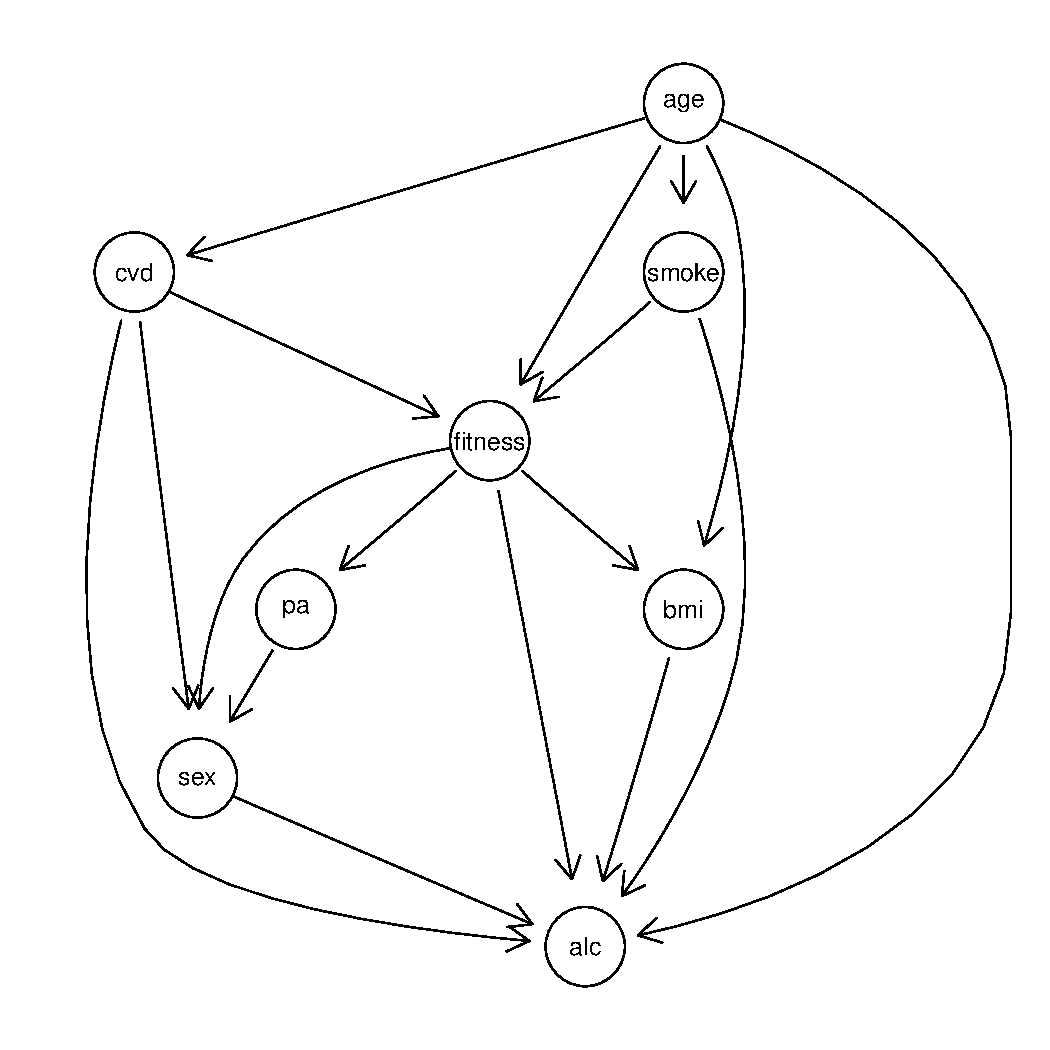
\includegraphics[width=\maxwidth]{figure/Rete_Bayesiana-1} 
\end{knitrout}
  
  La rete mostra degli archi non realistici, per esempio abbiamo che le variabili
  FITNESS e PA (Attività Fisica) influenzano in qualche modo la determinazione del
  SEX dell'individuo. Per risolvere questo problema dobbiamo generare una 
  gerarchia tra le variabili, tramite un loro ordinamento, in modo tale da non 
  avere incoerenze tra i vari archi. Nonostante ciò, è importante osservare
  come all'interno di questa rete è presente comunque una relazione tra le
  variabili FITNESS, SMOKE e ALCHOL.
  
  \subsection{Ordinamento delle Variabili}
    L'ordinamento che andrò ad utilizzare sarà:
    \begin{enumerate}
      \item Variabili di background: SEX, AGE
      \item Attività che influenzano il CVD: ALCHOL, SMOKE, PA
      \item Condizione fisica del paziente: BMI, FITNESS
      \item Variabile di risposta: CVD
    \end{enumerate}
    
\begin{knitrout}
\definecolor{shadecolor}{rgb}{0.969, 0.969, 0.969}\color{fgcolor}\begin{kframe}
\begin{alltt}
\hlcom{#Ordinamento delle variabili}
\hlcom{#1-SEX, 1-AGE, 3-BMI, 4-CVD, 3-FITNESS, 2-PA, 2-SMOKE, 2-ALC}
\hlcom{#Generazione matrice di adiacenza}
\hlstd{block}\hlkwb{<-}\hlkwd{c}\hlstd{(}\hlnum{1}\hlstd{,} \hlnum{1}\hlstd{,} \hlnum{3}\hlstd{,} \hlnum{4}\hlstd{,} \hlnum{3}\hlstd{,} \hlnum{2}\hlstd{,} \hlnum{2}\hlstd{,} \hlnum{2}\hlstd{)}
\hlstd{blnmc.bn} \hlkwb{<-} \hlkwd{matrix}\hlstd{(}\hlnum{0}\hlstd{,} \hlkwc{nrow}\hlstd{=}\hlnum{8}\hlstd{,} \hlkwc{ncol}\hlstd{=}\hlnum{8}\hlstd{)}
\hlkwd{rownames}\hlstd{(blnmc.bn)} \hlkwb{<-} \hlkwd{colnames}\hlstd{(blnmc.bn)} \hlkwb{<-} \hlkwd{names}\hlstd{(nmc.bn)}
\hlkwa{for} \hlstd{(b} \hlkwa{in} \hlnum{2}\hlopt{:}\hlnum{4}\hlstd{) blnmc.bn[block}\hlopt{==}\hlstd{b, block}\hlopt{<}\hlstd{b]} \hlkwb{<-} \hlnum{1}
\hlstd{blackL} \hlkwb{<-} \hlkwd{data.frame}\hlstd{(}\hlkwd{get.edgelist}\hlstd{(}\hlkwd{as}\hlstd{(blnmc.bn,} \hlstr{"igraph"}\hlstd{)))}
\hlkwd{names}\hlstd{(blackL)} \hlkwb{<-} \hlkwd{c}\hlstd{(}\hlstr{"from"}\hlstd{,} \hlstr{"to"}\hlstd{)}
\end{alltt}
\end{kframe}
\end{knitrout}
    
\begin{knitrout}
\definecolor{shadecolor}{rgb}{0.969, 0.969, 0.969}\color{fgcolor}\begin{kframe}
\begin{alltt}
\hlcom{#Rete Bayesiana gerarchica}
\hlstd{bn.o} \hlkwb{<-} \hlkwd{hc}\hlstd{(nmc.bn,} \hlkwc{blacklist}\hlstd{=blackL)}
\hlkwd{plot}\hlstd{(}\hlkwd{as}\hlstd{(}\hlkwd{amat}\hlstd{(bn.o),} \hlstr{"graphNEL"}\hlstd{))}
\end{alltt}
\end{kframe}
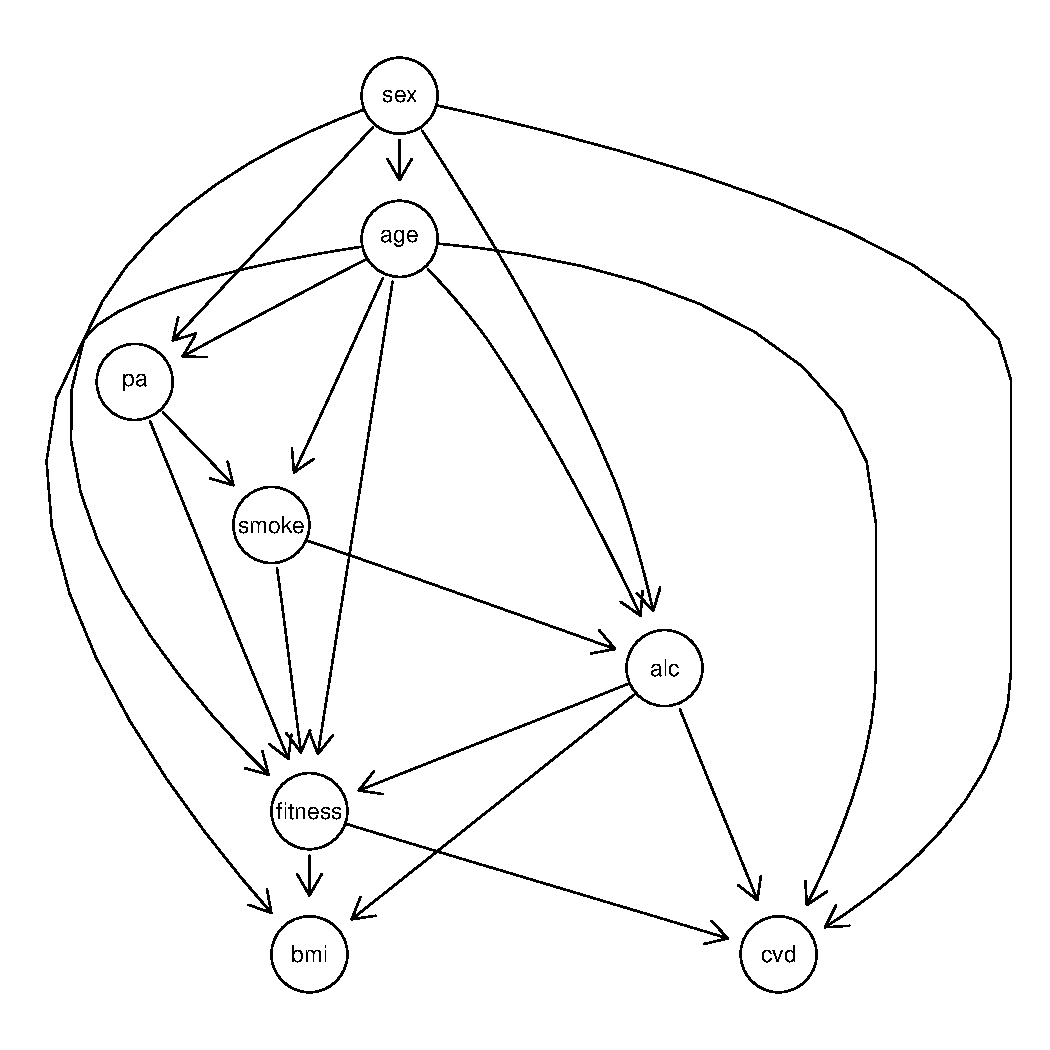
\includegraphics[width=\maxwidth]{figure/Rete_bayesiana_gerarchica-1} 
\end{knitrout}
    
    Anche in questo caso la rete con gerarchia mostra un incongruenza cioè la
    relazione diretta della variabile SEX sulla variabile AGE, come se il sesso 
    dell'individuo possa essere influenzato dalla sua età. Per questo motivo, 
    rimuoviamo quest arco e rieseguiamo la funzione hc.
    
\begin{knitrout}
\definecolor{shadecolor}{rgb}{0.969, 0.969, 0.969}\color{fgcolor}\begin{kframe}
\begin{alltt}
\hlcom{#Rimozione arco tra SEX e AGE}
\hlstd{block}\hlkwb{<-}\hlkwd{c}\hlstd{(}\hlnum{1}\hlstd{,} \hlnum{1}\hlstd{,} \hlnum{3}\hlstd{,} \hlnum{4}\hlstd{,} \hlnum{3}\hlstd{,} \hlnum{2}\hlstd{,} \hlnum{2}\hlstd{,} \hlnum{2}\hlstd{)}
\hlstd{blnmc.bn} \hlkwb{<-} \hlkwd{matrix}\hlstd{(}\hlnum{0}\hlstd{,} \hlkwc{nrow}\hlstd{=}\hlnum{8}\hlstd{,} \hlkwc{ncol}\hlstd{=}\hlnum{8}\hlstd{)}
\hlkwd{rownames}\hlstd{(blnmc.bn)} \hlkwb{<-} \hlkwd{colnames}\hlstd{(blnmc.bn)} \hlkwb{<-} \hlkwd{names}\hlstd{(nmc.bn)}
\hlkwa{for} \hlstd{(b} \hlkwa{in} \hlnum{2}\hlopt{:}\hlnum{4}\hlstd{) blnmc.bn[block}\hlopt{==}\hlstd{b, block}\hlopt{<}\hlstd{b]} \hlkwb{<-} \hlnum{1}
\hlcom{#Vincolo tra Sex e Age}
\hlstd{blnmc.bn[}\hlnum{1}\hlstd{,}\hlnum{2}\hlstd{]} \hlkwb{=} \hlnum{1}
\hlstd{blnmc.bn[}\hlnum{2}\hlstd{,}\hlnum{1}\hlstd{]} \hlkwb{=} \hlnum{1}
\hlstd{blackL} \hlkwb{<-} \hlkwd{data.frame}\hlstd{(}\hlkwd{get.edgelist}\hlstd{(}\hlkwd{as}\hlstd{(blnmc.bn,} \hlstr{"igraph"}\hlstd{)))}
\hlkwd{names}\hlstd{(blackL)} \hlkwb{<-} \hlkwd{c}\hlstd{(}\hlstr{"from"}\hlstd{,} \hlstr{"to"}\hlstd{)}
\end{alltt}
\end{kframe}
\end{knitrout}
  
\begin{knitrout}
\definecolor{shadecolor}{rgb}{0.969, 0.969, 0.969}\color{fgcolor}\begin{kframe}
\begin{alltt}
\hlcom{#Bayesian Network}
\hlstd{m.bn} \hlkwb{<-} \hlkwd{hc}\hlstd{(nmc.bn,} \hlkwc{blacklist}\hlstd{=blackL)}
\hlkwd{plot}\hlstd{(}\hlkwd{as}\hlstd{(}\hlkwd{amat}\hlstd{(m.bn),} \hlstr{"graphNEL"}\hlstd{))}
\end{alltt}
\end{kframe}
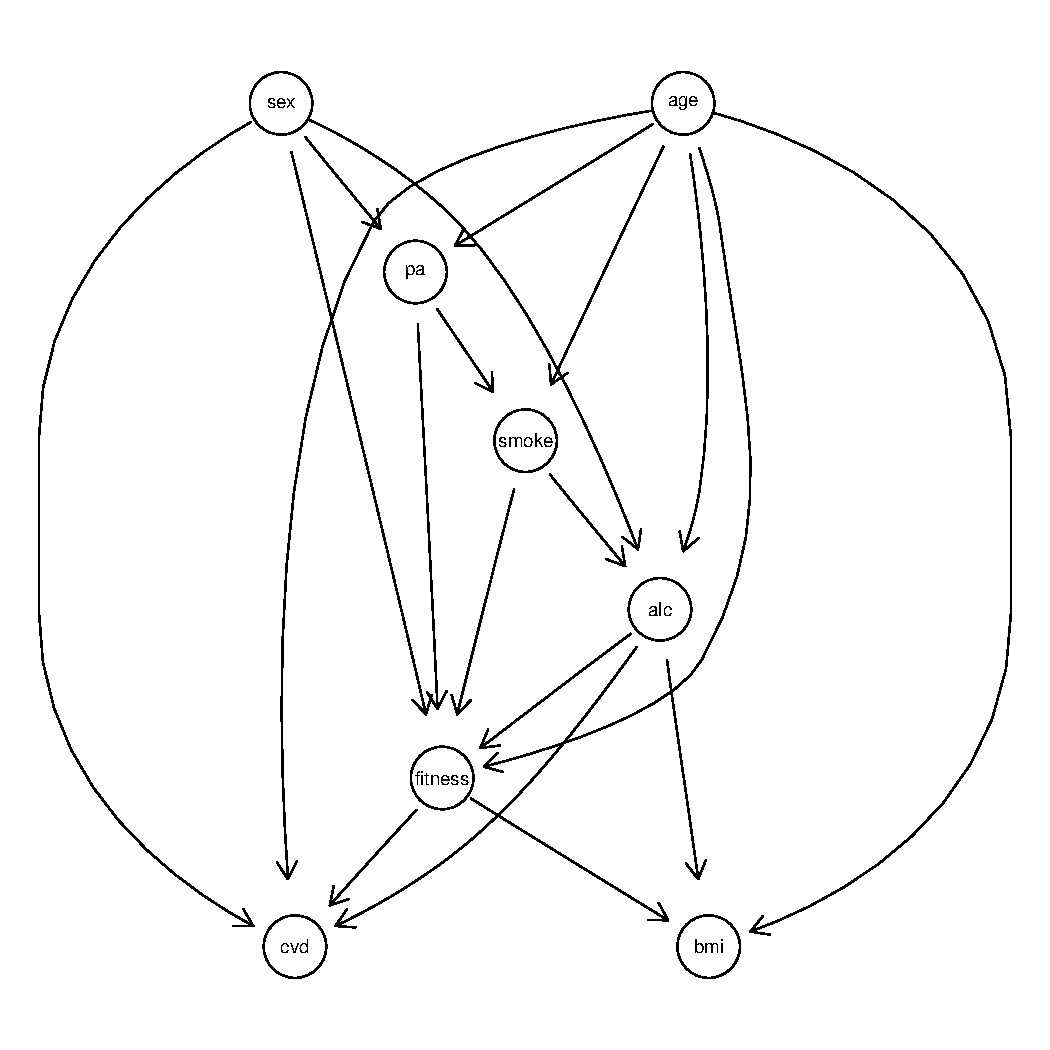
\includegraphics[width=\maxwidth]{figure/Bayesian_Network_finale-1} 
\end{knitrout}
    
    In questa ultima rete notiamo come è ancora presente le relazioni dirette
    delle variabili AGE, SEX, FITNESS e ALCHOL sulla variabile di risposta CVD. 
    Viceversa la CVD sembra non dipendere direttamente dalle variabili SMOKE, PA
    e BMI, ma per esempio la FITNESS è direttamente connessa con le variabili 
    PA, SMOKE e ALCHOL.
    
  \clearpage


\section{Considerazioni sul Modello}
  Date le reti e le analisi fatte precedentemente, effettuiamo adesso qualche
  considerazione su un possibile modello per la valutazione delle cause nella
  comparsa di una malattia cardiovascolare.
  
  \subsection{Fitness e PA}
    Abbiamo visto nelle precedenti reti come le variabili FITNESS e PA fossero 
    direttamente connessa tra di loro. Effettuiamo una regressione lineare per
    valutare l'effetto di PA sulla variabile FITNESS. 
    
\begin{knitrout}
\definecolor{shadecolor}{rgb}{0.969, 0.969, 0.969}\color{fgcolor}\begin{kframe}
\begin{alltt}
\hlcom{#Regressione Lineare tra Fitness e PA}
\hlstd{fit.fitness} \hlkwb{<-} \hlkwd{lm}\hlstd{(fitness}\hlopt{~}\hlstd{pa,} \hlkwc{data}\hlstd{=nmc)}
\hlkwd{summary}\hlstd{(fit.fitness)}
\end{alltt}
\begin{verbatim}
## 
## Call:
## lm(formula = fitness ~ pa, data = nmc)
## 
## Residuals:
##     Min      1Q  Median      3Q     Max 
## -2.5208 -0.5208  0.3059  0.4792  2.3059 
## 
## Coefficients:
##              Estimate Std. Error t value Pr(>|t|)    
## (Intercept)  3.520836   0.005101  690.22   <2e-16 ***
## pa          -0.826748   0.018934  -43.66   <2e-16 ***
## ---
## Signif. codes:  0 '***' 0.001 '**' 0.01 '*' 0.05 '.' 0.1 ' ' 1
## 
## Residual standard error: 0.8968 on 33325 degrees of freedom
## Multiple R-squared:  0.05412,	Adjusted R-squared:  0.05409 
## F-statistic:  1907 on 1 and 33325 DF,  p-value: < 2.2e-16
\end{verbatim}
\end{kframe}
\end{knitrout}
    
    Come è possibile vedere dalla semplice regressione lineare, l'attività
    fisica influisce positivamente nello stato di salute dell'individuo.
    Visualizziamo tramite un Barplot come le due variabili si dividono
    all'interno del Dataset osservato.
    
\begin{knitrout}
\definecolor{shadecolor}{rgb}{0.969, 0.969, 0.969}\color{fgcolor}\begin{kframe}
\begin{alltt}
\hlcom{#Barplot Fitness e PA}
\hlkwd{barplot}\hlstd{(}\hlkwd{table}\hlstd{(nmc}\hlopt{$}\hlstd{fitness, nmc}\hlopt{$}\hlstd{pa),}
        \hlkwc{names.arg}\hlstd{=}\hlkwd{c}\hlstd{(}\hlstr{"Attività Fisica"}\hlstd{,} \hlstr{"Non Attività Fisica"}\hlstd{),}
        \hlkwc{legend.text}\hlstd{=}\hlkwd{c}\hlstd{(}\hlstr{"Much Worse"}\hlstd{,} \hlstr{"Little Worse"}\hlstd{,}\hlstr{"Just as good"}\hlstd{,}
                \hlstr{"A bit better"}\hlstd{,} \hlstr{"Much better"}\hlstd{),}
        \hlkwc{col}\hlstd{=}\hlkwd{c}\hlstd{(black,red,orange,yellow,green),} \hlkwc{beside}\hlstd{=}\hlnum{TRUE}\hlstd{)}
\end{alltt}
\end{kframe}
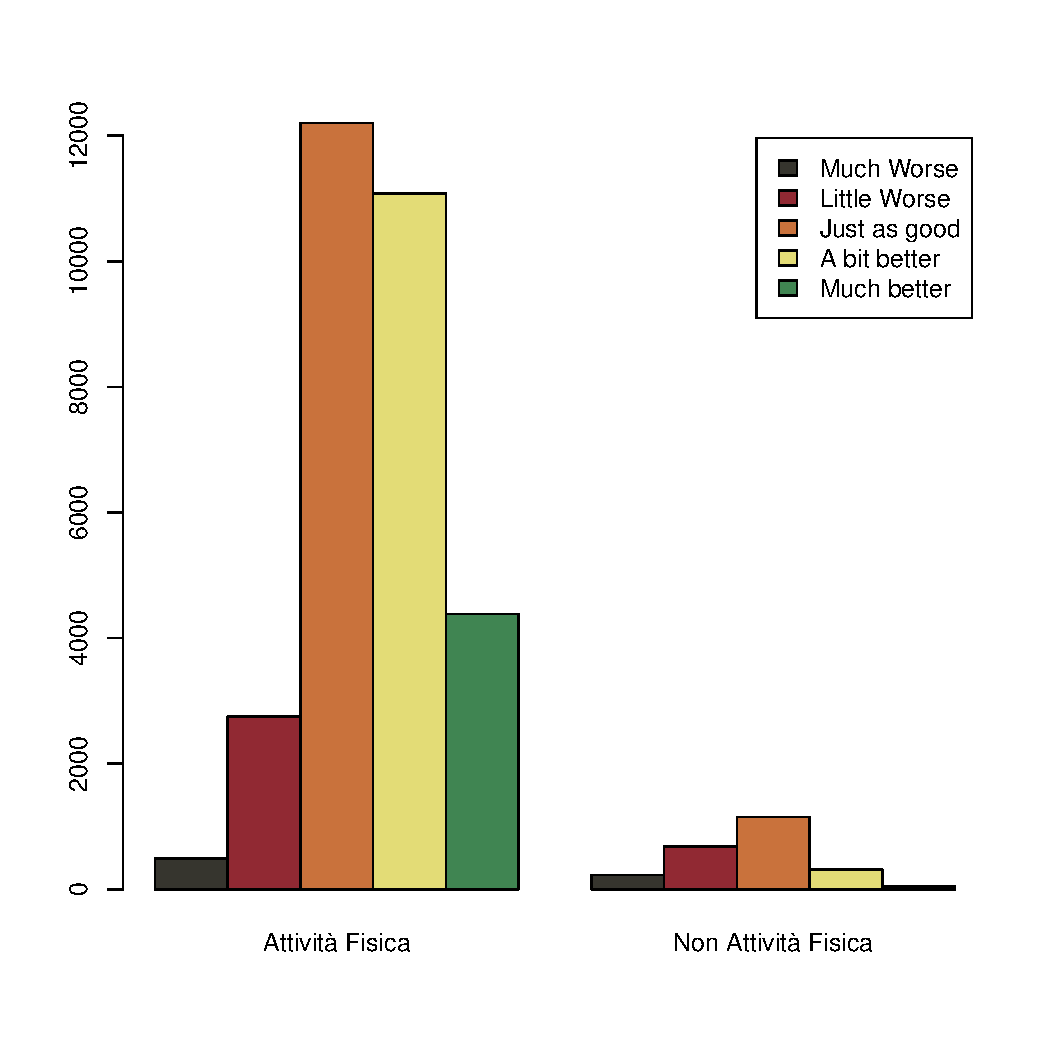
\includegraphics[width=\maxwidth]{figure/Barplot_Fitness_PA-1} 
\end{knitrout}
      
    Possiamo vedere nel Barplot come, all'interno del campione osservato,
    ci sia un aumento delle persone che hanno una miglior condizione di salute
    facendo attività fisica rispetto a chi non la pratica.
    Come detto precedentemente, dato che la variabile FITNESS è una variabile
    a carattere soggettivo dell'individuo e che questa è influenzata dalla
    variabile PA, verifichiamo come si potrebbe comportare quest ultima variabile
    all'interno di una rete bayesiana senza la presenza della variabile FITNESS,
    tenendo comunque conto della gerarchia e dei vincoli delle variabili fatto
    precedentemente.
    
\begin{knitrout}
\definecolor{shadecolor}{rgb}{0.969, 0.969, 0.969}\color{fgcolor}\begin{kframe}
\begin{alltt}
\hlcom{#Rete Bayesiana senza Fitness}
\hlcom{#Rimozione variabile Fitness}
\hlstd{nmc.bn} \hlkwb{=} \hlkwd{subset}\hlstd{(nmc.bn,} \hlkwc{select}\hlstd{=}\hlopt{-}\hlkwd{c}\hlstd{(fitness))}
\hlcom{#1-SEX, 1-AGE, 3-BMI, 4-CVD, 2-PA, 2-SMOKE, 2-ALC}
\hlstd{block}\hlkwb{<-}\hlkwd{c}\hlstd{(}\hlnum{1}\hlstd{,} \hlnum{1}\hlstd{,} \hlnum{3}\hlstd{,} \hlnum{4}\hlstd{,} \hlnum{2}\hlstd{,} \hlnum{2}\hlstd{,} \hlnum{2}\hlstd{)}
\hlstd{blnmc.bn} \hlkwb{<-} \hlkwd{matrix}\hlstd{(}\hlnum{0}\hlstd{,} \hlkwc{nrow}\hlstd{=}\hlnum{7}\hlstd{,} \hlkwc{ncol}\hlstd{=}\hlnum{7}\hlstd{)}
\hlkwd{rownames}\hlstd{(blnmc.bn)} \hlkwb{<-} \hlkwd{colnames}\hlstd{(blnmc.bn)} \hlkwb{<-} \hlkwd{names}\hlstd{(nmc.bn)}
\hlkwa{for} \hlstd{(b} \hlkwa{in} \hlnum{2}\hlopt{:}\hlnum{4}\hlstd{) blnmc.bn[block}\hlopt{==}\hlstd{b, block}\hlopt{<}\hlstd{b]} \hlkwb{<-} \hlnum{1}
\hlcom{#Vincolo tra Sex e Age}
\hlstd{blnmc.bn[}\hlnum{1}\hlstd{,}\hlnum{2}\hlstd{]} \hlkwb{=} \hlnum{1}
\hlstd{blnmc.bn[}\hlnum{2}\hlstd{,}\hlnum{1}\hlstd{]} \hlkwb{=} \hlnum{1}
\hlstd{blackL} \hlkwb{<-} \hlkwd{data.frame}\hlstd{(}\hlkwd{get.edgelist}\hlstd{(}\hlkwd{as}\hlstd{(blnmc.bn,} \hlstr{"igraph"}\hlstd{)))}
\hlkwd{names}\hlstd{(blackL)} \hlkwb{<-} \hlkwd{c}\hlstd{(}\hlstr{"from"}\hlstd{,} \hlstr{"to"}\hlstd{)}
\hlstd{m.bn} \hlkwb{<-} \hlkwd{hc}\hlstd{(nmc.bn,} \hlkwc{blacklist}\hlstd{=blackL)}
\hlkwd{plot}\hlstd{(}\hlkwd{as}\hlstd{(}\hlkwd{amat}\hlstd{(m.bn),} \hlstr{"graphNEL"}\hlstd{))}
\end{alltt}
\end{kframe}
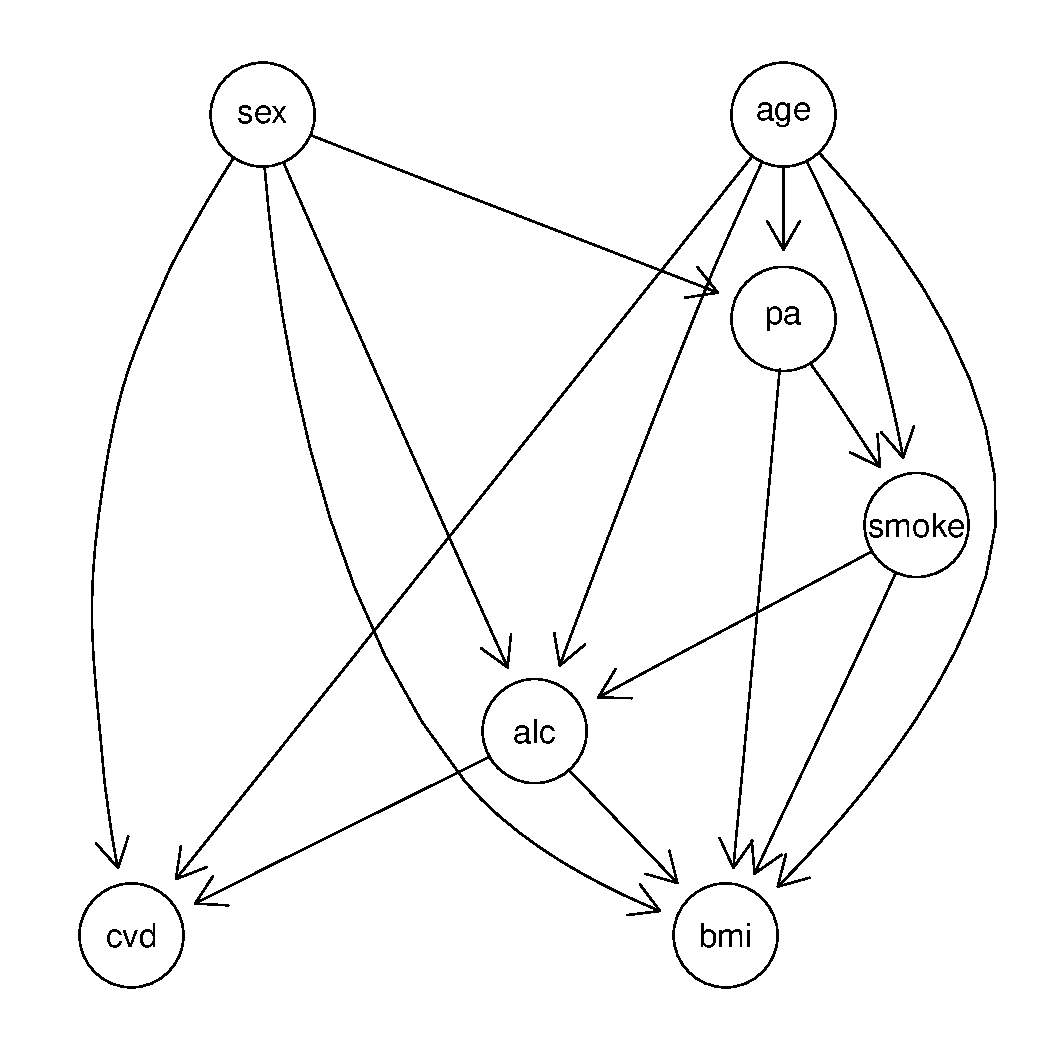
\includegraphics[width=\maxwidth]{figure/Rete_Bayesiana_senza_Fitness-1} 
\end{knitrout}
    
    In questa rete la variabile di risposta CVD è ancora direttamente connessa 
    con le variabili SEX, AGE e ALCHOL. La variabile PA, invece, influenza la
    la variabile SMOKE. La variabile BMI è anche influenzata dalle variabili 
    PA, ALCHOL, SMOKE, AGE e SEX.
  
  \subsection{BMI}
    Analizziamo ora, tramite una regressione logistica, l'influenza che hanno le
    variabili SEX, AGE, PA, ALC e SMOKE con la variabile BMI.
    
\begin{knitrout}
\definecolor{shadecolor}{rgb}{0.969, 0.969, 0.969}\color{fgcolor}\begin{kframe}
\begin{alltt}
\hlcom{#RLM per BMI}
\hlstd{fit.bmi} \hlkwb{<-} \hlkwd{glm}\hlstd{(bmi}\hlopt{~}\hlstd{sex}\hlopt{+}\hlstd{age}\hlopt{+}\hlstd{pa}\hlopt{+}\hlstd{smoke.ord}\hlopt{+}\hlstd{alc,} \hlkwc{family}\hlstd{=binomial,} \hlkwc{data}\hlstd{=nmc)}
\hlkwd{summary}\hlstd{(fit.bmi)}
\end{alltt}
\begin{verbatim}
## 
## Call:
## glm(formula = bmi ~ sex + age + pa + smoke.ord + alc, family = binomial, 
##     data = nmc)
## 
## Deviance Residuals: 
##     Min       1Q   Median       3Q      Max  
## -0.8170  -0.4024  -0.3567  -0.3181   2.7488  
## 
## Coefficients:
##              Estimate Std. Error z value Pr(>|z|)    
## (Intercept) -2.926869   0.104871 -27.909  < 2e-16 ***
## sexMale     -0.324341   0.049706  -6.525 6.79e-11 ***
## age          0.011322   0.001377   8.220  < 2e-16 ***
## pa           0.758050   0.066422  11.413  < 2e-16 ***
## smoke.ord    0.213703   0.033352   6.407 1.48e-10 ***
## alc         -0.235959   0.032115  -7.347 2.02e-13 ***
## ---
## Signif. codes:  0 '***' 0.001 '**' 0.01 '*' 0.05 '.' 0.1 ' ' 1
## 
## (Dispersion parameter for binomial family taken to be 1)
## 
##     Null deviance: 16621  on 33326  degrees of freedom
## Residual deviance: 16319  on 33321  degrees of freedom
## AIC: 16331
## 
## Number of Fisher Scoring iterations: 5
\end{verbatim}
\end{kframe}
\end{knitrout}
    
    \begin{itemize}
      \item Le variabili SEX, AGE, PA, ALC e SMOKE risultano tutte significative.
      \item Essere maschio influenza positivamente il BMI rispetto alla donna.
      \item L'età fa aumenta l'indice di BMI.
      \item Fare attività fisica riduce il BMI.
      \item Fumare fa aumentare l'indice BMI.
      \item Il consumo di alchol sembra diminuire l'indice BMI.
    \end{itemize}
    
    Contrariamente a quello che ci si potesse aspettare, sembrerebbe che un
    maggior consumo di alchol possa diminuire l'indice di massa corporea,
    visualizziamo quindi, tramite Barplot, come si distribuiscono le persone in 
    base all'indice di BMI e al consumo di alchol all'interno del Dataset.
    
\begin{knitrout}
\definecolor{shadecolor}{rgb}{0.969, 0.969, 0.969}\color{fgcolor}\begin{kframe}
\begin{alltt}
\hlcom{#Barplot per BMI e Alchol}
\hlkwd{barplot}\hlstd{(}\hlkwd{table}\hlstd{(nmc}\hlopt{$}\hlstd{bmi, nmc}\hlopt{$}\hlstd{alc),}
        \hlkwc{names.arg}\hlstd{=}\hlkwd{c}\hlstd{(}\hlstr{"Nessun"}\hlstd{,}\hlstr{"Poco"}\hlstd{,}\hlstr{"Medio"}\hlstd{,}\hlstr{"Alto"}\hlstd{),}
        \hlkwc{legend.text}\hlstd{=}\hlkwd{c}\hlstd{(}\hlstr{"BMI Basso"}\hlstd{,} \hlstr{"BMI Alto"}\hlstd{),}
        \hlkwc{col}\hlstd{=}\hlkwd{c}\hlstd{(}\hlstr{"#408552"}\hlstd{,} \hlstr{"#912933"}\hlstd{),} \hlkwc{beside}\hlstd{=}\hlnum{TRUE}\hlstd{)}
\end{alltt}
\end{kframe}
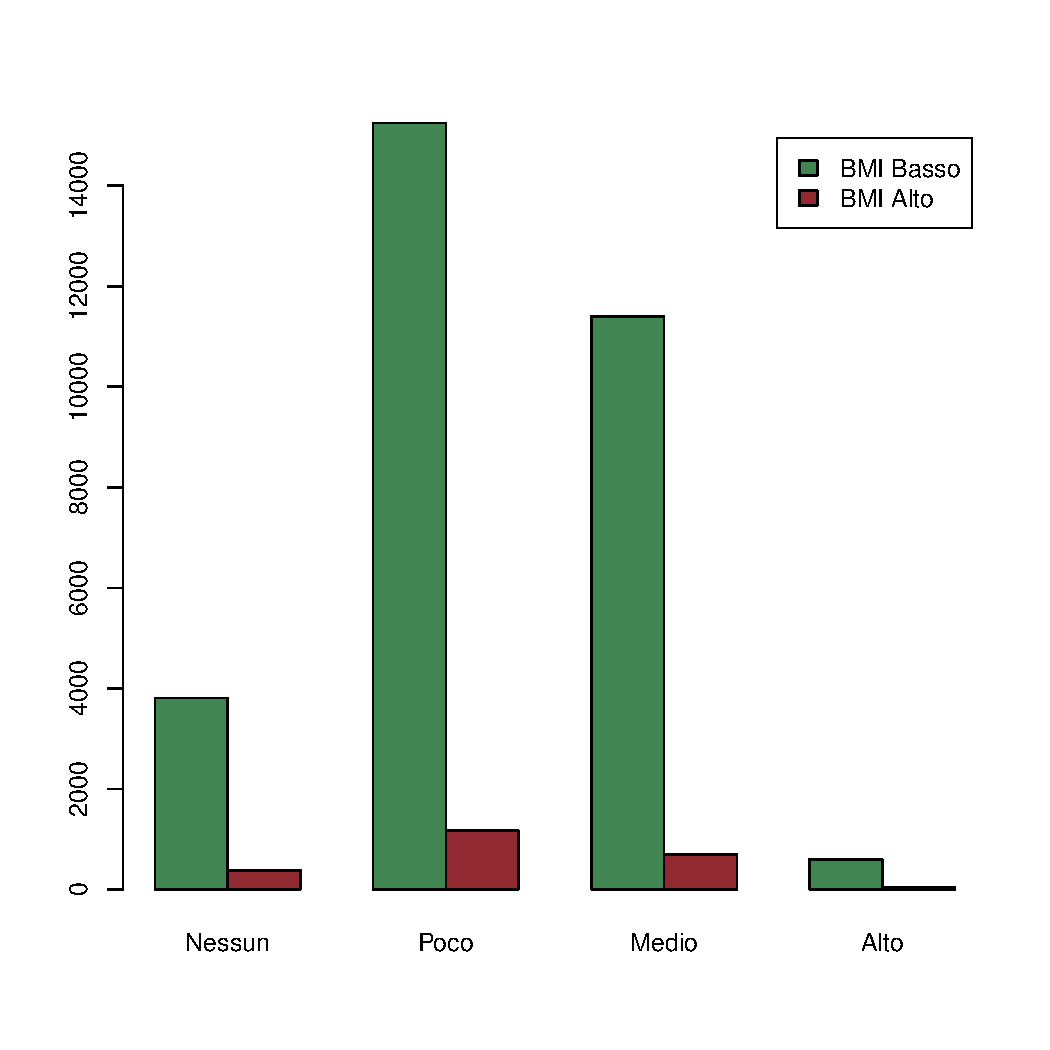
\includegraphics[width=\maxwidth]{figure/Barplot_BMI_e_Alchol-1} 
\end{knitrout}
    
    Possiamo vedere come ci sia una prevalenza di persone con basso indice BMI 
    per ogni categoria di consumatori di alchol rispetto alle persone con un 
    alto indice di BMI.
    Proviamo a togliere la variabile ALCHOL nella regressione logistica di BMI 
    se il modello risulta ancora significativo.
    
\begin{knitrout}
\definecolor{shadecolor}{rgb}{0.969, 0.969, 0.969}\color{fgcolor}\begin{kframe}
\begin{alltt}
\hlcom{#RLM per BMI senza Alchol}
\hlstd{fit.bmi.nalc} \hlkwb{<-} \hlkwd{glm}\hlstd{(bmi}\hlopt{~}\hlstd{sex}\hlopt{+}\hlstd{age}\hlopt{+}\hlstd{pa}\hlopt{+}\hlstd{smoke.ord,} \hlkwc{family}\hlstd{=binomial,} \hlkwc{data}\hlstd{=nmc)}
\hlkwd{summary}\hlstd{(fit.bmi.nalc)}
\end{alltt}
\begin{verbatim}
## 
## Call:
## glm(formula = bmi ~ sex + age + pa + smoke.ord, family = binomial, 
##     data = nmc)
## 
## Deviance Residuals: 
##     Min       1Q   Median       3Q      Max  
## -0.6986  -0.4001  -0.3627  -0.3209   2.5988  
## 
## Coefficients:
##              Estimate Std. Error z value Pr(>|z|)    
## (Intercept) -3.341359   0.089561 -37.308  < 2e-16 ***
## sexMale     -0.379425   0.049150  -7.720 1.17e-14 ***
## age          0.010972   0.001392   7.880 3.28e-15 ***
## pa           0.765789   0.066320  11.547  < 2e-16 ***
## smoke.ord    0.159274   0.032623   4.882 1.05e-06 ***
## ---
## Signif. codes:  0 '***' 0.001 '**' 0.01 '*' 0.05 '.' 0.1 ' ' 1
## 
## (Dispersion parameter for binomial family taken to be 1)
## 
##     Null deviance: 16621  on 33326  degrees of freedom
## Residual deviance: 16373  on 33322  degrees of freedom
## AIC: 16383
## 
## Number of Fisher Scoring iterations: 5
\end{verbatim}
\end{kframe}
\end{knitrout}
    
    Anche senza la presenza della variabile ALCHOL, questo modello per BMI
    risulta significativo non modificando di molto il comportamento delle altre 
    variabili. Per questo motivo, rimuoviamo l'arco che va dalla variabile
    ALCHOL a BMI.
    
\begin{knitrout}
\definecolor{shadecolor}{rgb}{0.969, 0.969, 0.969}\color{fgcolor}\begin{kframe}
\begin{alltt}
\hlcom{#Rete Bayesiana senza arco da Alchol a BMI}
\hlstd{m.bn.bmicvd} \hlkwb{<-} \hlkwd{DAG}\hlstd{(cvd}\hlopt{~}\hlstd{sex}\hlopt{:}\hlstd{age}\hlopt{:}\hlstd{alc, alc}\hlopt{~}\hlstd{sex}\hlopt{:}\hlstd{age}\hlopt{:}\hlstd{smoke, smoke}\hlopt{~}\hlstd{pa}\hlopt{:}\hlstd{age,}
                   \hlstd{pa}\hlopt{~}\hlstd{sex}\hlopt{:}\hlstd{age, bmi}\hlopt{~}\hlstd{sex}\hlopt{:}\hlstd{pa}\hlopt{:}\hlstd{age}\hlopt{:}\hlstd{smoke)}
\hlkwd{plot}\hlstd{(}\hlkwd{as}\hlstd{(m.bn.bmicvd,} \hlstr{"graphNEL"}\hlstd{))}
\end{alltt}
\end{kframe}
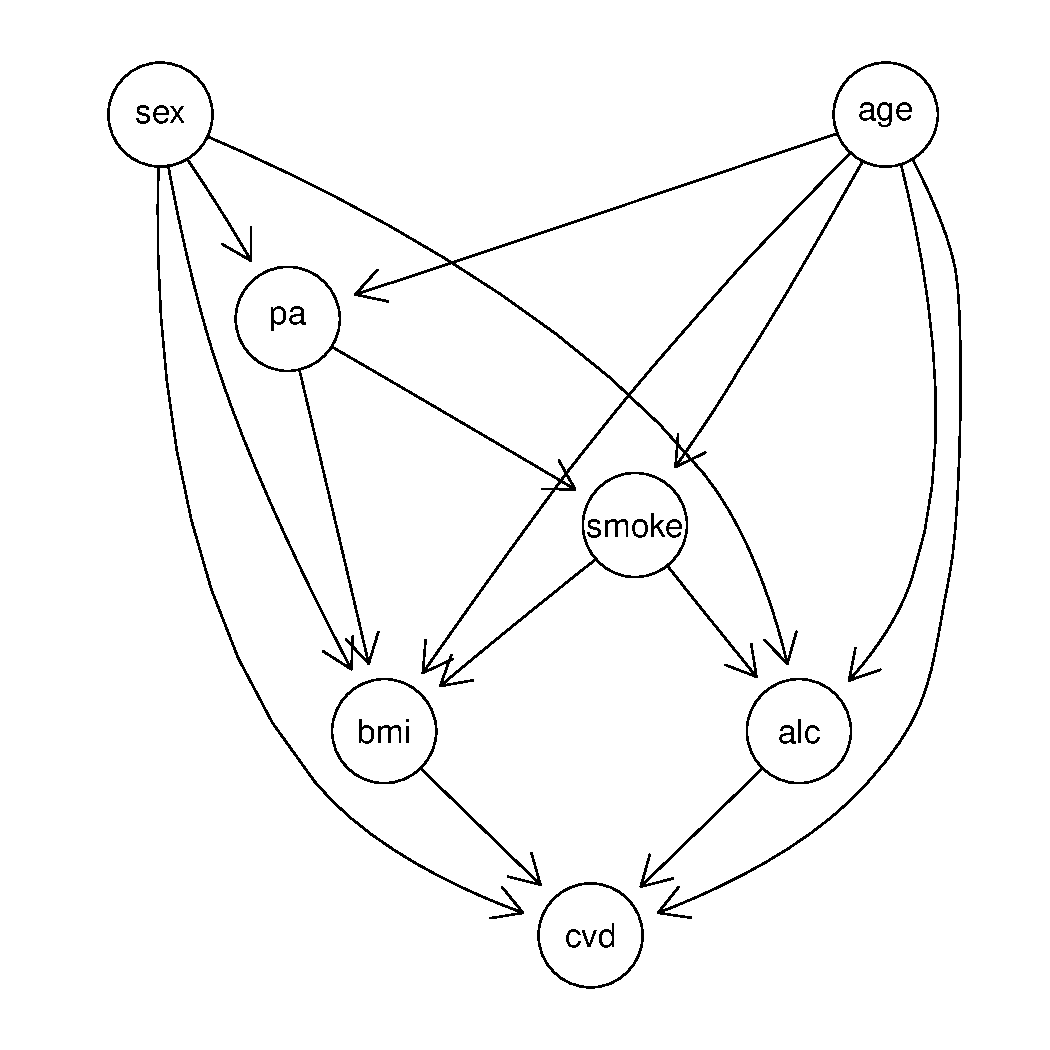
\includegraphics[width=\maxwidth]{figure/Rete_Bayesiana_senza_arco_tra_Alchol_e_BMI-1} 
\end{knitrout}
    
    Nell'analisi delle regressioni logistiche abbiamo notato anche come un aumento 
    dell'indice di massa corporea sia direttamente connessa all'insorgenza di 
    malattie cardiovascolari, per questo motivo andremo ad aggiungere nella rete
    un arco che va dalla variabile BMI alla variabile di risposta CVD.
    
\begin{knitrout}
\definecolor{shadecolor}{rgb}{0.969, 0.969, 0.969}\color{fgcolor}\begin{kframe}
\begin{alltt}
\hlcom{#Rete Bayesiana con arco da BMI a CVD}
\hlstd{m.bn.bmicvd} \hlkwb{<-} \hlkwd{DAG}\hlstd{(cvd}\hlopt{~}\hlstd{sex}\hlopt{:}\hlstd{age}\hlopt{:}\hlstd{alc}\hlopt{:}\hlstd{bmi,alc}\hlopt{~}\hlstd{sex}\hlopt{:}\hlstd{age}\hlopt{:}\hlstd{smoke,smoke}\hlopt{~}\hlstd{pa}\hlopt{:}\hlstd{age,}
                   \hlstd{pa}\hlopt{~}\hlstd{sex}\hlopt{:}\hlstd{age, bmi}\hlopt{~}\hlstd{sex}\hlopt{:}\hlstd{pa}\hlopt{:}\hlstd{age}\hlopt{:}\hlstd{smoke)}
\hlkwd{plot}\hlstd{(}\hlkwd{as}\hlstd{(m.bn.bmicvd,} \hlstr{"graphNEL"}\hlstd{))}
\end{alltt}
\end{kframe}
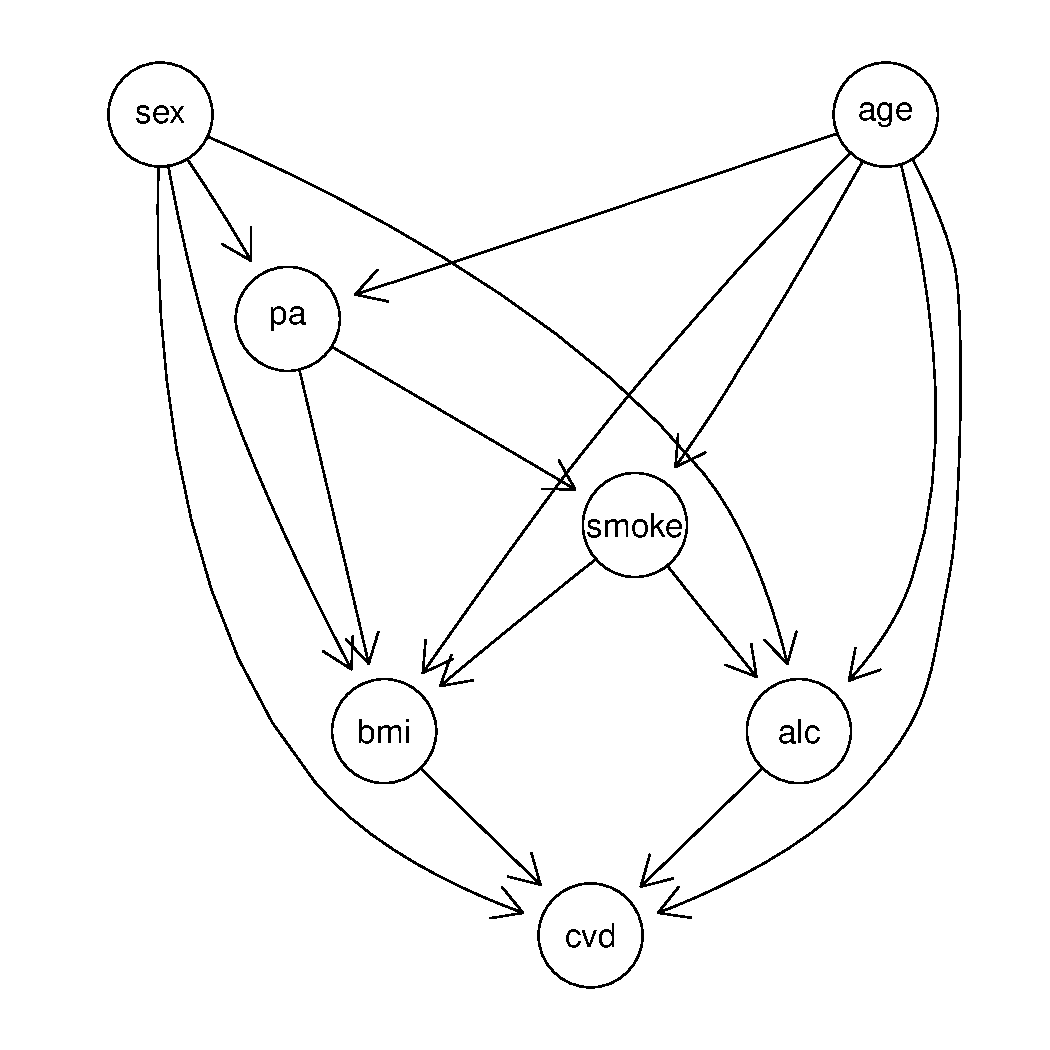
\includegraphics[width=\maxwidth]{figure/Rete_Bayesiana_con_arco_BMI_-__CVD-1} 
\end{knitrout}
    
  \subsection{Alchol}
    Sempre durante l'analisi delle regressioni logistiche e durante la 
    visualizzazione dei grafi non orientati, abbiamo visto come la variabile 
    ALCHOL non influenzi direttamente la variabile di risposta CVD. Per questo
    motivo andremo a rimuovere l'arco da ALCHOL a CVD dato che è presente all'
    interno della rete.
    
\begin{knitrout}
\definecolor{shadecolor}{rgb}{0.969, 0.969, 0.969}\color{fgcolor}\begin{kframe}
\begin{alltt}
\hlcom{#Rete Bayesiana senza arco da Alchol a CVD}
\hlstd{m.bn.bmicvd} \hlkwb{<-} \hlkwd{DAG}\hlstd{(cvd}\hlopt{~}\hlstd{sex}\hlopt{:}\hlstd{age}\hlopt{:}\hlstd{bmi, alc}\hlopt{~}\hlstd{sex}\hlopt{:}\hlstd{age}\hlopt{:}\hlstd{smoke, smoke}\hlopt{~}\hlstd{pa}\hlopt{:}\hlstd{age,}
                   \hlstd{pa}\hlopt{~}\hlstd{sex}\hlopt{:}\hlstd{age, bmi}\hlopt{~}\hlstd{sex}\hlopt{:}\hlstd{pa}\hlopt{:}\hlstd{age}\hlopt{:}\hlstd{smoke)}
\hlkwd{plot}\hlstd{(}\hlkwd{as}\hlstd{(m.bn.bmicvd,} \hlstr{"graphNEL"}\hlstd{))}
\end{alltt}
\end{kframe}
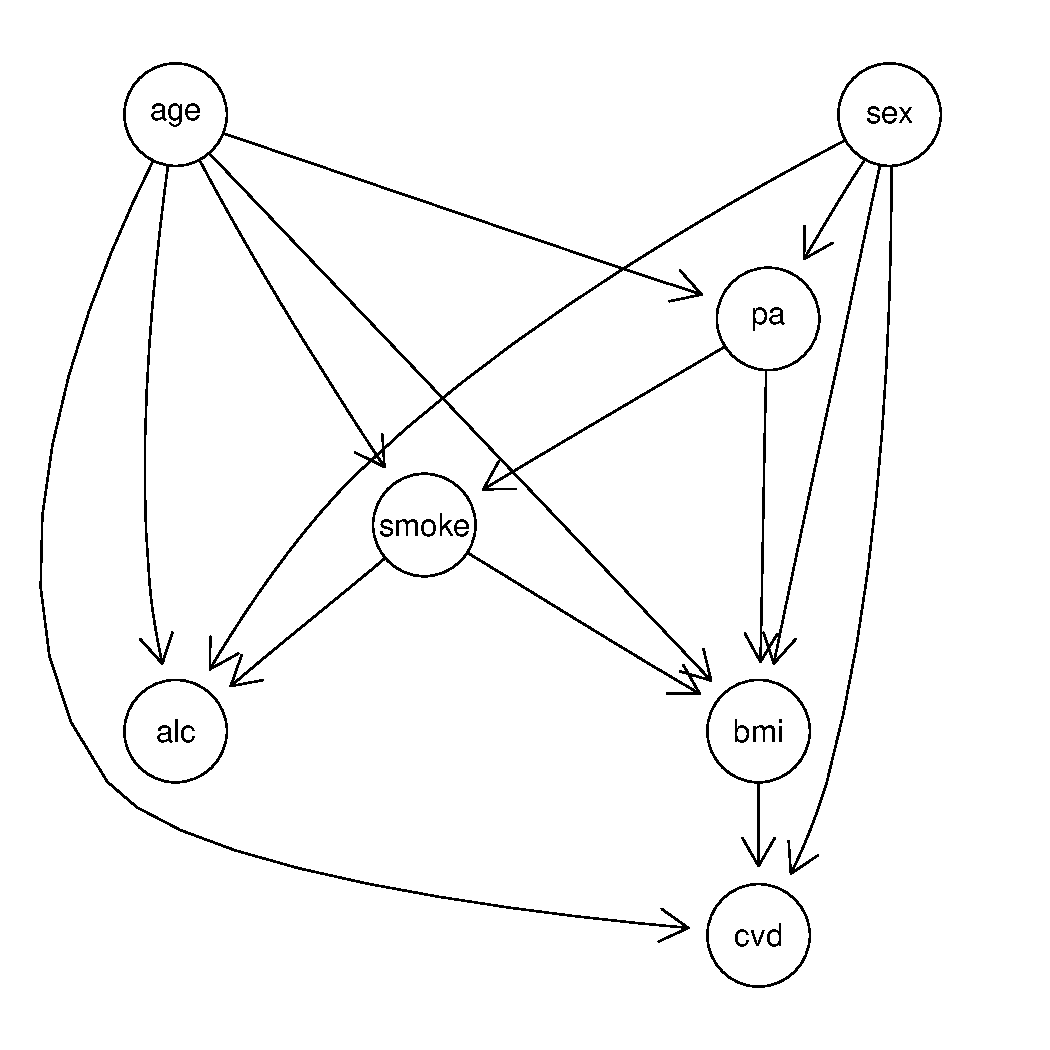
\includegraphics[width=\maxwidth]{figure/Rete_Bayesiana_senza_arco_tra_Alchol_e_CVD-1} 
\end{knitrout}
    
    Valutiamo ora le dipendenze di Alchol tramite la regressione lineare.
    
\begin{knitrout}
\definecolor{shadecolor}{rgb}{0.969, 0.969, 0.969}\color{fgcolor}\begin{kframe}
\begin{alltt}
\hlcom{#RLM per Alchol}
\hlstd{fit.alc} \hlkwb{<-} \hlkwd{lm}\hlstd{(alc}\hlopt{~}\hlstd{sex}\hlopt{+}\hlstd{age}\hlopt{+}\hlstd{smoke.ord,} \hlkwc{data}\hlstd{=nmc)}
\hlkwd{summary}\hlstd{(fit.alc)}
\end{alltt}
\begin{verbatim}
## 
## Call:
## lm(formula = alc ~ sex + age + smoke.ord, data = nmc)
## 
## Residuals:
##      Min       1Q   Median       3Q      Max 
## -1.89216 -0.34663 -0.08867  0.62980  1.98374 
## 
## Coefficients:
##             Estimate Std. Error t value Pr(>|t|)    
## (Intercept) 1.728132   0.014122  122.37   <2e-16 ***
## sexMale     0.236272   0.007822   30.21   <2e-16 ***
## age         0.003017   0.000226   13.35   <2e-16 ***
## smoke.ord   0.227791   0.005795   39.31   <2e-16 ***
## ---
## Signif. codes:  0 '***' 0.001 '**' 0.01 '*' 0.05 '.' 0.1 ' ' 1
## 
## Residual standard error: 0.6726 on 33323 degrees of freedom
## Multiple R-squared:  0.07519,	Adjusted R-squared:  0.07511 
## F-statistic: 903.1 on 3 and 33323 DF,  p-value: < 2.2e-16
\end{verbatim}
\end{kframe}
\end{knitrout}
    
    Dal modello per ALCHOL vediamo che:
    \begin{itemize}
      \item Gli uomini fanno più consumo di alchol rispetto alle donne.
      \item Con l'aumentare dell'età si aumenta anche il consumo di alcoli.
      \item Chi fuma tende a fare un consumo maggiore di alcolici.
    \end{itemize}
    
  \subsection{Smoke}
    Andiamo ora a valutare le dipendenze che ha la variabile SMOKE tramite
    la regressione lineare.
    
\begin{knitrout}
\definecolor{shadecolor}{rgb}{0.969, 0.969, 0.969}\color{fgcolor}\begin{kframe}
\begin{alltt}
\hlcom{#RLM per Smoke}
\hlstd{fit.smoke} \hlkwb{<-} \hlkwd{lm}\hlstd{(smoke.ord}\hlopt{~}\hlstd{age}\hlopt{+}\hlstd{pa,} \hlkwc{data}\hlstd{=nmc)}
\hlkwd{summary}\hlstd{(fit.smoke)}
\end{alltt}
\begin{verbatim}
## 
## Call:
## lm(formula = smoke.ord ~ age + pa, data = nmc)
## 
## Residuals:
##     Min      1Q  Median      3Q     Max 
## -0.5415 -0.4235 -0.4034  0.5765  1.6059 
## 
## Coefficients:
##              Estimate Std. Error t value Pr(>|t|)    
## (Intercept) 1.3785578  0.0108812 126.691  < 2e-16 ***
## age         0.0007751  0.0002133   3.633  0.00028 ***
## pa          0.0908136  0.0134240   6.765 1.36e-11 ***
## ---
## Signif. codes:  0 '***' 0.001 '**' 0.01 '*' 0.05 '.' 0.1 ' ' 1
## 
## Residual standard error: 0.6353 on 33324 degrees of freedom
## Multiple R-squared:  0.001711,	Adjusted R-squared:  0.001652 
## F-statistic: 28.57 on 2 and 33324 DF,  p-value: 4.026e-13
\end{verbatim}
\end{kframe}
\end{knitrout}
    
    Dal modello per SMOKE vediamo che:
    \begin{itemize}
      \item Con l'aumentare dell'età si tende a fumare di più.
      \item Chi non fa attività fisica tende a fumare di più.
    \end{itemize}
    
  \subsection{Sex:Male e Sex:Female}
    Durante le precedenti analisi, abbiamo notato come ci sia una probabilità 
    maggiore del sesso maschile rispetto a quello femminile della comparsa di
    CVD.
    Valutiamo se ci sono differenze nelle due reti bayesiane, una per il
    genere maschile e l'altra per quella femminile.
    
\begin{knitrout}
\definecolor{shadecolor}{rgb}{0.969, 0.969, 0.969}\color{fgcolor}\begin{kframe}
\begin{alltt}
\hlcom{#Dataset: sotto-problema Sex}
\hlstd{male} \hlkwb{<-} \hlstd{(nmc.bn}\hlopt{$}\hlstd{sex}\hlopt{==}\hlnum{1}\hlstd{)}
\hlstd{female} \hlkwb{<-} \hlstd{(nmc.bn}\hlopt{$}\hlstd{sex}\hlopt{==}\hlnum{0}\hlstd{)}
\hlstd{nmc.bn.male} \hlkwb{<-} \hlstd{nmc.bn[male,} \hlkwd{c}\hlstd{(}\hlnum{2}\hlopt{:}\hlnum{7}\hlstd{)]}
\hlstd{nmc.bn.female} \hlkwb{<-} \hlstd{nmc.bn[female,} \hlkwd{c}\hlstd{(}\hlnum{2}\hlopt{:}\hlnum{7}\hlstd{)]}
\end{alltt}
\end{kframe}
\end{knitrout}
    
\begin{knitrout}
\definecolor{shadecolor}{rgb}{0.969, 0.969, 0.969}\color{fgcolor}\begin{kframe}
\begin{alltt}
\hlcom{#Rete Bayesiana per Male}
\hlcom{#1-AGE, 3-BMI, 4-CVD, 2-PA, 2-SMOKE, 2-ALC}
\hlstd{block}\hlkwb{<-}\hlkwd{c}\hlstd{(}\hlnum{1}\hlstd{,} \hlnum{3}\hlstd{,} \hlnum{4}\hlstd{,} \hlnum{2}\hlstd{,} \hlnum{2}\hlstd{,} \hlnum{2}\hlstd{)}
\hlstd{blnmc.bn} \hlkwb{<-} \hlkwd{matrix}\hlstd{(}\hlnum{0}\hlstd{,} \hlkwc{nrow}\hlstd{=}\hlnum{6}\hlstd{,} \hlkwc{ncol}\hlstd{=}\hlnum{6}\hlstd{)}
\hlkwd{rownames}\hlstd{(blnmc.bn)} \hlkwb{<-} \hlkwd{colnames}\hlstd{(blnmc.bn)} \hlkwb{<-} \hlkwd{names}\hlstd{(nmc.bn.male)}
\hlkwa{for} \hlstd{(b} \hlkwa{in} \hlnum{2}\hlopt{:}\hlnum{4}\hlstd{) blnmc.bn[block}\hlopt{==}\hlstd{b, block}\hlopt{<}\hlstd{b]} \hlkwb{<-} \hlnum{1}
\hlstd{blnmc.bn[}\hlnum{1}\hlstd{,}\hlnum{2}\hlstd{]} \hlkwb{=} \hlnum{1}
\hlstd{blnmc.bn[}\hlnum{2}\hlstd{,}\hlnum{1}\hlstd{]} \hlkwb{=} \hlnum{1}
\hlstd{blackL} \hlkwb{<-} \hlkwd{data.frame}\hlstd{(}\hlkwd{get.edgelist}\hlstd{(}\hlkwd{as}\hlstd{(blnmc.bn,} \hlstr{"igraph"}\hlstd{)))}
\hlkwd{names}\hlstd{(blackL)} \hlkwb{<-} \hlkwd{c}\hlstd{(}\hlstr{"from"}\hlstd{,} \hlstr{"to"}\hlstd{)}
\hlstd{m.bn.male} \hlkwb{<-} \hlkwd{hc}\hlstd{(nmc.bn.male,} \hlkwc{blacklist}\hlstd{=blackL)}
\hlkwd{plot}\hlstd{(}\hlkwd{as}\hlstd{(}\hlkwd{amat}\hlstd{(m.bn.male),} \hlstr{"graphNEL"}\hlstd{))}
\end{alltt}
\end{kframe}
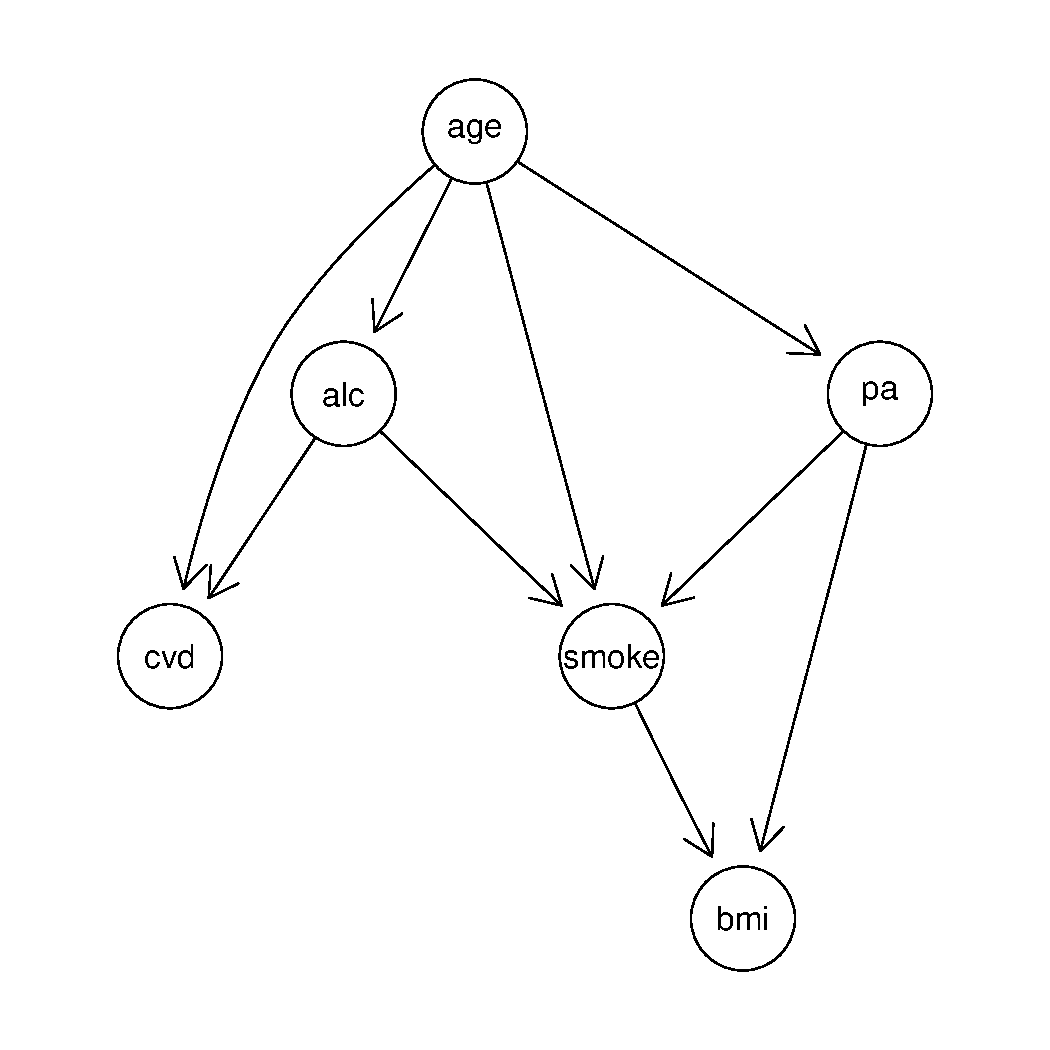
\includegraphics[width=\maxwidth]{figure/Rete_Bayesiana_per_Male-1} 
\end{knitrout}
    
    
\begin{knitrout}
\definecolor{shadecolor}{rgb}{0.969, 0.969, 0.969}\color{fgcolor}\begin{kframe}
\begin{alltt}
\hlcom{#Rete Bayesiana per Female}
\hlcom{#1-AGE, 3-BMI, 4-CVD, 2-PA, 2-SMOKE, 2-ALC}
\hlstd{block}\hlkwb{<-}\hlkwd{c}\hlstd{(}\hlnum{1}\hlstd{,} \hlnum{3}\hlstd{,} \hlnum{4}\hlstd{,} \hlnum{2}\hlstd{,} \hlnum{2}\hlstd{,} \hlnum{2}\hlstd{)}
\hlstd{blnmc.bn} \hlkwb{<-} \hlkwd{matrix}\hlstd{(}\hlnum{0}\hlstd{,} \hlkwc{nrow}\hlstd{=}\hlnum{6}\hlstd{,} \hlkwc{ncol}\hlstd{=}\hlnum{6}\hlstd{)}
\hlkwd{rownames}\hlstd{(blnmc.bn)} \hlkwb{<-} \hlkwd{colnames}\hlstd{(blnmc.bn)} \hlkwb{<-} \hlkwd{names}\hlstd{(nmc.bn.female)}
\hlkwa{for} \hlstd{(b} \hlkwa{in} \hlnum{2}\hlopt{:}\hlnum{4}\hlstd{) blnmc.bn[block}\hlopt{==}\hlstd{b, block}\hlopt{<}\hlstd{b]} \hlkwb{<-} \hlnum{1}
\hlstd{blnmc.bn[}\hlnum{1}\hlstd{,}\hlnum{2}\hlstd{]} \hlkwb{=} \hlnum{1}
\hlstd{blnmc.bn[}\hlnum{2}\hlstd{,}\hlnum{1}\hlstd{]} \hlkwb{=} \hlnum{1}
\hlstd{blackL} \hlkwb{<-} \hlkwd{data.frame}\hlstd{(}\hlkwd{get.edgelist}\hlstd{(}\hlkwd{as}\hlstd{(blnmc.bn,} \hlstr{"igraph"}\hlstd{)))}
\hlkwd{names}\hlstd{(blackL)} \hlkwb{<-} \hlkwd{c}\hlstd{(}\hlstr{"from"}\hlstd{,} \hlstr{"to"}\hlstd{)}
\hlstd{m.bn.female} \hlkwb{<-} \hlkwd{hc}\hlstd{(nmc.bn.female,} \hlkwc{blacklist}\hlstd{=blackL)}
\hlkwd{plot}\hlstd{(}\hlkwd{as}\hlstd{(}\hlkwd{amat}\hlstd{(m.bn.female),} \hlstr{"graphNEL"}\hlstd{))}
\end{alltt}
\end{kframe}
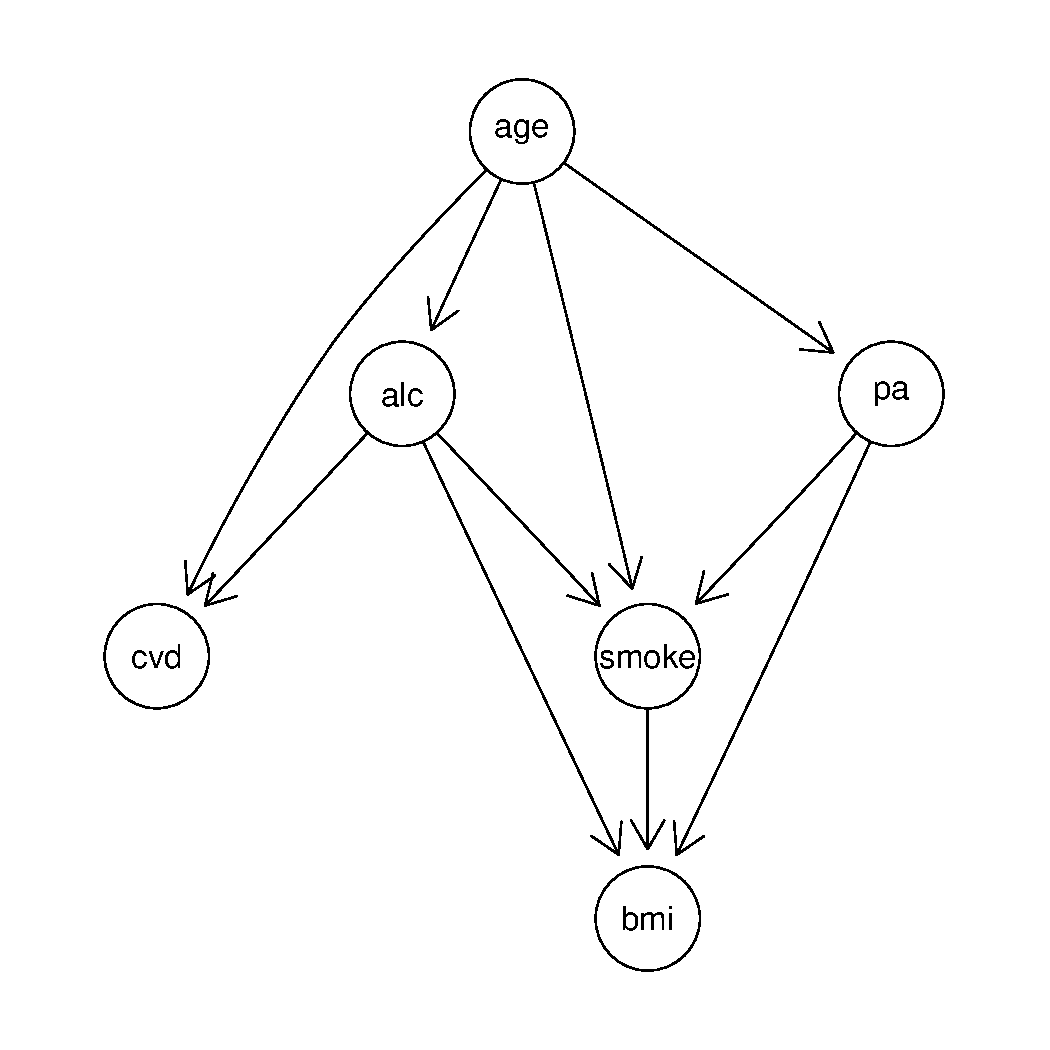
\includegraphics[width=\maxwidth]{figure/Rete_Bayesiana_per_Female-1} 
\end{knitrout}
    
    Le reti non presentano particolari differenze tranne nella rete del genere 
    maschile dove è presente l'arco che va da ALCHOL a BMI. Se non consideriamo 
    quest arco per quello che abbiamo detto precedentemente (con l'aggiunta
    anche della diretta connessione che la BMI ha su la CVD) le due reti risultano
    identiche.
      
\clearpage


\section{Conclusioni}
  In conclusione, il modello scelto che più si adatta meglio alla comprensione
  e alle cause di un problema cardiovascolare è:\\
  Modello: CVD $\sim$ SEX + AGE + BMI \par
  Infatti i fattori che aumentano la probabilità di CVD sono:
  \begin{itemize}
    \item Essere maschio.
    \item L'aumento dell'età.
    \item Avere un alto indice di massa corporea.
  \end{itemize}
  Il fatto età però risulta particolarmente rilevante superata la soglia dei 40
  anni, mostrando come la malattia si manifesti sopratutto nella fascia
  più anziana della popolazione. L'uso della sigaretta può far aumentare 
  l'indice di massa corporea che è un fattore scatenante della CVD. Per quanto
  visto, per ridurre l'indice di massa corporea, è consigliabile fare attività.
  

\end{document}
